\chapter{A Substantial Improvement to Ceccato et al.’s Framework}
\label{chap:proposal}

\linenumbers
\lettrine[lines=2]{I}{n Chapter \ref{state_of_art}}, we presented the state of the art of \textit{process comprehension} of an Industrial Control System (ICS) with a focus on the methodology proposed by Ceccato et al. \cite{ceccato}[Section \ref{sec:3_ceccato_metodology}], explaining what it consists of, its practical application on a testbed, and most importantly highlighting its limitations and critical issues (see Section \ref{subsec:3_ceccato_limitations}).

\bigskip
In this chapter we will present \textbf{a proposal to improve the methodology} presented in the previous chapter, addressing most of the critical issues (or at least trying to do so) mentioned above by almost completely rewriting the original framework, enhancing its functionalities and inserting new ones where possible, while preserving its general structure and approach. The system analysis will in fact consist of the same four steps as in the original methodology (Data Pre-processing, Graph and Statistical Analysis, Business Process Mining and Invariants Inference), but each of them will be deeply revised in order to provide a richer, clearer and more complete process comprehension of the industrial system to be analyzed and its behavior.

\bigskip
As it may have already been noted, my proposals do not involve improving the data gathering phase: this is due simply to the fact that the novel framework will not be tested on the same case study used by Ceccato et, al. (Section \ref{subsec:3_testbed}), but on a different case study, the ITrust SWaT system \cite{swat_home}, of which (some) datasets containing the execution trace of the physical system and the network traffic scan are already provided by iTrust itself. For more details about this case study, the reader is referred to Chapter \ref{casestudy}.

\section{The Proposed New Framework}
\label{sec:4_framework_presentation}
In our version of the framework we decided to follow a few design choices:

\begin{enumerate}
	\item it must be implemented in a \textbf{single programming language};
	\item it must be \textbf{independent of the system} to be analyzed;
	\item It must provide greater \textbf{flexibility and ease of use} for the user at every stage.
\end{enumerate}
In the following, we discuss these three features in more detail.

\begin{description}
	\item[Single Programming Language] The original tool was implemented using various programming languages in each of the different phases: from Python up to Java, passing through Bash scripting. \newline
	In our opinion, this heterogeneity makes it more difficult and less intuitive for the user to operate on the tool: moreover, the use of multiple technologies makes it more difficult to maintain the code and add new features, particularly if only a single person is managing the code (he/she might be proficient in one language, but little of the others).
	
	\bigskip
	For these reasons, we decided to use a single programming language, to ensure homogeneity to the framework and ease of use and maintenance of the code for anyone who wants to manage it in the future: we chose to use Python, because of its simplicity and easy readability combined with its versatility and powerfulness: moreover, Python can count on a massive number of available libraries and packages that meet all kinds of needs.
	
	\item[System Independence] One of the biggest limitations of Ceccato et al.'s tool that we highlighted in Section \ref{subsec:3_ceccato_limitations} is the fact that it is \textbf{highly dependent on the testbed used}: that is, it is \textit{not} possible to configure any of the tool's parameters to analyze different industrial systems.\newline
	To overcome this issue and make my framework independent of the system to be analyzed, also eliminating all references to hardcoded variables and values present in the previous tool, we decided to use a \textbf{general configuration file}, named \textit{config.ini}, in which the user can, at will, customize all the parameters necessary to perform the analysis of the targeted system.
	
	\item[Flexibility and Ease on Use] The lack of flexibility and ease of use in a tool can be a significant disadvantage, limiting its effectiveness and making it challenging for the user to get the desired outcomes. The original tool suffered from these limitations, with users having to run scripts from the command line, with little to no options or parameters available to customize the analysis. As a result, the tool was not user-friendly and lacked the flexibility to adapt to specific user needs. 
	
	\bigskip
	To settle these issues, I enhanced the command-line interface in the novel framework by adding new options and parameters. These new features provide the user with greater flexibility, enabling to specify parameters and options that allow for more in-depth analysis and focused results analyzing data more effectively and efficiently. With these enhancements, the framework has become more user-friendly, reducing the learning curve and making it more accessible to a wider range of users. \newline
	This, in turn, makes the framework more valuable and useful, increasing its adoption and effectiveness across a range of industrial control systems and applications. \newline
	Moreover, with new options and parameters users no longer have to rely solely on the command line interface, which can be challenging and intimidating for those with limited technical expertise. Instead, users can now access a range of customizable options and parameters, making the tool more intuitive and user-friendly. 
\end{description}
Overall, the enhancements made to the framework represent a significant step forward in making it more effective, efficient, and user-friendly.


%\paragraph{General Configuration File \textit{config.ini}} 
%The configuration file \textit{config.ini} for the framework I am %presenting in this thesis is intended, as mentioned, to make it %customizable in order to fit a variety of different systems and allow 
%for their analysis. Here the user can configure general parameters and %options, such as paths to read from or write files to, or related to %individual analysis phases.\newline
%The file is divided into sections, each covering a different aspect of 
%the configuration: each section contains user-customizable constants 
%that will then be called within the Python scripts that constitute the %framework. An example can be appreciated in Listing %\ref{lst:config_ini_example}:

%\begin{lstlisting}[language=bash, numbers=none, caption=Example of %\textit{config.ini} file, label=lst:config_ini_example]	
%	[PATHS]
%	root_dir = /home/marcuzzo/UniVr/Tesi
%	project_dir = %(root_dir)s/PLC-RE
%	input_dataset_directory = %(root_dir)s/datasets_SWaT/2015
%	net_csv_path = %(root_dir)s/datasets_SWaT/2015/Network_CSV
%	
%	[DEFAULTS]
%	dataset_file = PLC_SWaT_Dataset.csv
%	granularity = 10
%	number_of_rows = 20000
%	skip_rows = 100000
%	
%	[DAIKON]
%	daikon_dir = daikon
%	daikon_invariants_dir = %(daikon_dir)s/Daikon_Invariants
%	daikon_results_dir = %(daikon_invariants_dir)s/results
%	daikon_results_file_original = daikon_results_full.txt
%	inv_conditions_file = Inv_conditions.spinfo
%	max_security_pct_margin = 1
%	min_security_pct_margin = 2
%	
%	...
%\end{lstlisting}

\subsection{Framework Structure}
\label{subsec:4_framework_struct}
The structure of the novel framework mostly follows the structure of the original tool: it is divided into four main directories each representing the different phases of the analysis (data pre-processing, graphs and statistical analysis, process mining, and invariant analysis), and containing the relevant Python scripts that perform the analysis, as well as subdirectories and any input/output files necessary for the proper behavior of the framework.

\begin{lstlisting}[language=bash, numbers=none, caption=Novel Framework structure and Python scripts, label=lst:4_tree_command]
	.
	├── config.ini
	├── daikon
	│   ├── Daikon_Invariants
	│   ├── daikonAnalysis.py
	│   └── runDaikon.py
	├── network-analysis
	│   ├── data
	│   ├── networkAnalysis.py
	│   ├── export_pcap_data.py
	│   └── swat_csv_extractor.py
	├── pre-processing
	│   ├── mergeDatasets.py
	│   └── system_info.py
	├── process-mining
	│   ├── data
	│   └── process_mining.py
	└── statistical-graphs
	    ├── histPlots_Stats.py
	    └── runChartSubPlots.py
\end{lstlisting}

Ahead of these directories there is the most important part, that allows the framework to be independent of the industrial control system being analyzed: the \textit{config.ini} file. Here the user can configure general parameters and options, such as paths to read from or write files to, or related to individual analysis phases.\newline
The file is divided into sections, each covering a different aspect of 
the configuration: each section contains user-customizable parameters 
that will then be called within the Python scripts that constitute the framework. Sections of \textit{config.ini} are:

\begin{itemize}
	\item \textbf{[PATHS]:} defines general paths such as the project root directory and some source directories for datasets;
	
	\item \textbf{[PREPROC]:} contains some parameters needed for the pre-processing phase;
	
	\item \textbf{[DATASET]:} defines settings and parameters used during the dataset enrichment stage and possibly in further phases;
	
	\item \textbf{[DAIKON]:} defines parameters needed for invariant analysis with Daikon;
	
	\item \textbf{[MINING]:} contains parameters used during the process mining phase;
	
	\item \textbf{[NETWORK]:} Contains specific settings for extracting the data obtained from the packet sniffing phase on the ICS network and converting it to CSV format. It also defines the network protocols that are to be analyzed.
\end{itemize}

\subsection{Python Libraries and External Tools}
\label{subsec:4_tools_libraries}
As the framework has been developed entirely in Python, the objective was to minimize reliance on external tools and instead integrate various functionalities within the framework itself. The aim was to make the framework independent from external software. The only remaining external tool from the Ceccato et al. tool is Daikon. This choice was made because there is currently no better alternative or Python package available that offers the same functionalities as Daikon.

\bigskip
Instead, the framework extensively utilizes Python libraries for handling various functionalities and input data. The core libraries on which the framework relies are:

\begin{itemize}
	\item \textbf{Pandas}, also used in the previous tool for dataset management, but whose use here has been deepened and extended	
	\item \textbf{NumPy}, often used together with Pandas to perform some operations to support it;
	
	\item \textbf{MatPlotLib}, for managing and plotting graphical analysis;
	
	\item other scientific libraries such as \textbf{SciPy}, \textbf{StatsModel} \cite{statsmodel} and \textbf{NetworkX} \cite{networkx}, for mathematical, statistical and analysis operations on the data;
	
	\item \textbf{GraphViz}, for the creation of activity diagrams in the process mining phase.
\end{itemize}
Having now seen the structure of the framework, in the next sections we will go into more detail describing our proposal.

\section{Analysis Phases}

\subsection{Phase 1: Data Pre-processing}
\label{subsec:improve_preprocessing}
\textit{Data Pre-processing phase} is probably the most delicate and significant one: depending on how large the industrial system to be analyzed is, the data collected, and how it is enriched using the additional attributes, the subsequent system analysis will provide more or less accurate outcomes.

\bigskip
The previous tool has several limitations, particularly at this stage. It does not allow for the isolation of a subsystem, either in terms of time or the number of PLCs to be analyzed. The system is considered as a whole without the ability to focus on specific subsystems. Additionally, many of the additional attributes had to be manually added, and for the ones entered automatically, there is no way to specify the register type to associate them with.\newline
The combination of these limitations, along with the presence of hardcoded references to attributes and registers in the tool's code, makes the analysis of the system more challenging. Furthermore, it compromises the accuracy and reliability of the obtained results in terms of both quantity and quality.

\bigskip
In the proposed framework, these issues have been addressed by incorporating new features. Firstly, the framework allows for the selection of a subsystem from the command line based on both temporal criteria and the specific PLCs to be included. This enables more focused and targeted analysis. Additionally, we have revamped the process of enriching the resulting dataset by eliminating manual entry of additional attributes. Instead, users now have the flexibility to determine the type of additional attribute to associate with a specific register.\newline
Furthermore, after the pre-processing stage, a preliminary analysis can be conducted on the resulting dataset. This analysis aims to identify the registers that are associated with actuators, measurements, and hardcoded setpoints or constants. It provides insights into the dataset and helps in refining the enrichment step. The parameters for this analysis can be configured in the \textit{config.ini} file, allowing for customization and fine-tuning of the process.\newline \newline 
In the upcoming sections, we will delve into a more comprehensive examination of the achievements made in this framework.
\vfill

\subsubsection{Subsystem Selection}
\label{subsubsec:4_select_subsystem}

In the previous tool, the datasets for each individual PLC in CSV format were required to be placed in a specific directory that was hardcoded in the script. The script would then merge and enrich these datasets to generate a single output dataset representing the complete process trace of the industrial system. However, the script did not provide options to select specific PLCs for analysis or define a temporal range for analysis. This lack of flexibility made the analysis more complex, especially when dealing with \textit{transient states} (i.e., general statea in which the industrial system is still initializing before actually reaching full operation) or when focusing on specific parts of the industrial system during certain periods of interest. The fixed dataset structure also may increase the number of variables that could be analyzed.\newline
Furthermore, the previous tool did not allow for specifying an output CSV file to save the resulting dataset. Each dataset creation and enrichment operation would overwrite the previous file, making it inconvenient for comparisons between different execution traces unless the files were manually renamed.

\bigskip
The proposed framework addressed these issues by introducing improvements. First of all, in the general \textit{config.ini} file there are some general default settings about paths, and among them the one concerning the directory where to place the datasets of the individual PLCs to be processed. In addition to this option, there are other ones that define further aspects related to the operations performed in this phase. Listing \ref{lst:config_ini_preproc} shows the settings in question: 

\begin{lstlisting}[language=bash, numbers=none, caption=Paths and parameters for the Pre-processing phase in \textit{config.ini} file, label=lst:config_ini_preproc]	
	[PATHS]
	root_dir = /home/marcuzzo/UniVr/Tesi
	project_dir = %(root_dir)s/PLC-RE
	net_csv_path = %(root_dir)s/datasets_SWaT/2015/Network_CSV
	
	[PREPROC]
	raw_dataset_directory = datasets_SWaT/2015 # Directory containg datasets
	dataset_file = PLC_SWaT_Dataset.csv # Default output dataset
	granularity = 10  # slope granularity
	number_of_rows = 20000  # Seconds to consider
	skip_rows = 100000  # Skip seconds from beginning
\end{lstlisting}
At the same time, the user has the option to specify these settings via the command line using the new Python script called \texttt{mergeDatasets.py}, located in the \texttt{pre-processing} directory of the project. Any options provided through the command line will override the default settings specified in the \textit{config.ini} file. These options are:

\begin{itemize}
	\item \textbf{-s} or \textbf{{-}{-}skiprows:} initial transient period (expressed in seconds) to be skipped. This option is useful in case the system has an initial transient or the analyzer wishes to start the analysis from a specific point in the dataset;
	
	\item \textbf{-n} or \textbf{{-}{-}nrows:} time interval under analysis, expressed in terms of the number of rows in the dataset.\newline
	This option makes a \textbf{selection} on the data of the dataset;
	
	\item \textbf{-p} or \textbf{{-}{-}plcs:} PLCs to be merged and enriched. The user can specify the desired PLCs by indicating the CSV file names of the associated datasets with no limitations on number.\newline
	This option makes a \textbf{projection} on the data of the dataset.
	
	\item \textbf{-d} or \textbf{{-}{-}directory:} performs the merge and enrichment of all CSV files contained in the directory specified by user, overriding the default setting in \textit{config.ini}. It is in fact the old functionality of the previous tool, maintained here to give the user more flexibility and convenience in case he wants to perform the analysis on the whole system. This is also the default behavior in case the \texttt{-p} option is not specified.
	
	\item \textbf{-o} or \textbf{{-}{-}output:} specifies the name of the file in which the obtained dataset will be saved. It must necessarily be a file in CSV format.
	
	\item \textbf{-g} or \textbf{{-}{-}granularity:} specifies a granularity (expressed in seconds) that will be used to calculate the measurement slope during the dataset enrichment phase. We will discuss this later in Section \ref{subsubsec:4_dataset_enrichment}.
\end{itemize}

\subsubsection{Dataset Enrichment}
\label{subsubsec:4_dataset_enrichment}
After a step in which a function is applied to each PLC-related dataset to eliminate its unused registers within the system \footnote{This is especially true if the Modbus register scan has been performed, in which ranges of registers are scanned: it is assumed that unused registers have constant value zero}, the \textbf{dataset enrichment operation} is performed.\newline
This operation differs from the previous version not only in the fact that it is performed on each individual dataset and not on the resulting dataset, but also in the additional attributes: not only are they greater in number, but they are automatically calculated and inserted by the \texttt{mergeDatasets.py} script into the dataset and, most importantly, it is possible to decide through the parameters in the \textit{config.ini} configuration file under the \texttt{[DATASET]} section to which registers these attributes should be assigned. \newline
In Listing \ref{lst:4_enrich_params} we can see the list of additional attributes and how they should be associated with the registers of the dataset:

\begin{lstlisting}[language=Python,numbers=none,caption={\texttt{config.ini} parameters for dataset enriching},label=lst:4_enrich_params]
	[DATASET]
	timestamp_col = Timestamp
	max_prefix = max_
	min_prefix = min_
	max_min_cols_list = lit|ait|dpit
	prev_cols_prefix = prev_
	prev_cols_list = mv[0-9]{3}|p[0-9]{3}
	trend_cols_prefix = trend_
	trend_cols_list = lit
	trend_period = 150
	slope_cols_prefix = slope_
	slope_cols_list = lit
\end{lstlisting}
Following is a brief explanation of the parameters just seen:

\begin{description}
	\item[\texttt{timestap\_col}] indicates the name of the column that contains the data timestamps. This parameter is used not only in this phase, but is also referred to in the Process Mining phase. In the previous work, this parameter was hardcoded and not configurable (and thus causing errors if the system being analyzed changed)
	
	\item[\texttt{max\_prefix}, \texttt{min\_prefix}, \texttt{max\_min\_cols\_list}] refer to any relative maximum or minimum values (\textit{relative setpoints}) of one or more measures and that can be found and inserted as new columns within the dataset. The first two parameters indicate the prefix to be used in the column names affected by this additional attribute, while the third specifies of which type of registers we want to know the maximum and/or minimum value reached (several options can be specified using the logical operator \texttt{|} - or).\newline 
	If, for example, we want to know the maximum value of the registers associated with the tanks, indicated in the iTrust SWaT system by the prefix \texttt{LIT}, we only need to specify the necessary parameter in the \textit{config.ini} file, so \texttt{max\_min\_cols\_list = lit}.\newline
	The result will be to have in the dataset thus enriched a new column named \texttt{max\_P1\_LIT101}.
	
	\item[\texttt{prev\_cols\_prefix}, \texttt{prev\_cols\_list}]  refer to the values at the previous time instant of the registers specified in \texttt{prev\_cols\_list}. It is possible to specify registers using \textit{regex}, as in the example shown. It may be useful in some cases to have this value available to check, for example, when a change of state of a single given actuator occurs.  The behavior of these parameters is the same as described in the point above.
	
	\item[\texttt{slope\_cols\_prefix}, \texttt{slope\_cols\_list}] are related to the calculation of the slope of a specific register (usually a measure), that is, its trend. The slope can be \textbf{ascending} (if its value is greater than zero), \textbf{descending} (if less than zero) or \textbf{stable} (if approximately equal to zero). We will delve into the details of slope calculation in the following paragraph, as it pertains to the attributes \texttt{trend\_cols\_prefix}, \texttt{trend\_cols\_list}, and \texttt{trend\_period}.
\end{description}

Initially, the parameters for registers to be associated with each additional attribute may be left blank, as we may not have prior knowledge about the system and are unsure about which registers correspond to actuators, measurements, or other attributes. This information can be obtained from the brief analysis that follows the merging of datasets. The analysis, performed based on user's choice, provides indications on potential sensors, actuators, and other relevant information. These indications help the user set the desired values in the \textit{config.ini} file and refine the enrichment process by re-launching the \texttt{mergeDatasets.py} script.

\paragraph{Slope Calculation}
The \textit{slope} is an attribute that represents the \textbf{trend} of the measurement being considered. It is particularly useful, in our context, during the inference and invariant analysis phase to gather information about the trend under specific conditions. The slope can generally be classified as \textbf{increasing} (slope > 0), \textbf{decreasing} (slope < 0), or \textbf{stable} (slope = 0).\newline
Normally, the slope is calculated through a simple mathematical formula: given an interval \textit{a}, \textit{b} relative to the measurement \textit{l}, the slope is given by the difference of these two values divided by the amount of time \textit{t} that the measurement takes to reach \textit{b} from \textit{a}:

\[slope = \frac{l(b) -l(a)}{t(b) - t(a)}\]

In the proposed framework, similar to the previous tool, this time interval (the granularity) can be adjusted to be either long or short. The choice of granularity depends on the desired accuracy of the slope calculation. A lower granularity will provide a slope that closely reflects the actual measurement trend, while a higher granularity will result in flatter slope data. Each time interval within which the measurement is divided corresponds to a slope value. These slopes are calculated and added as additional attributes in the dataset. Later on, these slope values are used to determine the trend of the measurement in specific situations or conditions.

\bigskip
Calculating the slope directly from the raw measurement data can be a suitable approach for systems where the measurements are not heavily influenced by \textbf{perturbations}. Perturbations, such as liquid oscillations in a tank during filling and emptying phases, can lead to fluctuating readings of the level. In such cases, maintaining a low granularity can provide a more accurate calculation of the overall trend that closely aligns with the actual measurement trend. The tanks of Ceccato et al.'s testbed are an example where this holds true.\newline
However, if perturbations significantly affect the measurement readings, calculating the slope on individual time intervals may result in an inaccurate trend definition, irrespective of the chosen granularity. In such cases, the fluctuating nature of the measurements due to perturbations can introduce errors in the slope calculation, making it less reliable as an indicator of the actual trend.

\bigskip
Figure \ref{fig:4_slope_comparison} demonstrates this assertion: the measurement, in blue, refers to the LIT101 tank of the iTrust SWaT system; in red, the slope calculation related to the measurement with three different granularities: 30 (Figure \ref{subfig:4_slope_g30_nodecomp}), 60 (Figure \ref{subfig:4_slope_g60_nodecomp}) and 120 seconds (Figure \ref{subfig:4_slope_g120_nodecomp}). It is noticeable that as the granularity increases, the slope values flatten. Moreover, in the time interval between seconds 1800 and 4200, the level of LIT101 exhibits a predominantly increasing trend, yet the calculated slope values fluctuate between positive and negative. Consequently, during the invariant analysis, the overall increasing trend may not be detected, resulting in a loss of information.\newline \newline
The previous tool did not take into account the possibility of having strongly perturbed data, which presented a challenge that we needed to address in the development of the proposed framework.
\vfill
\pagebreak

\begin{figure}[H]
	\centering
	\begin{subfigure}{0.9\textwidth}
		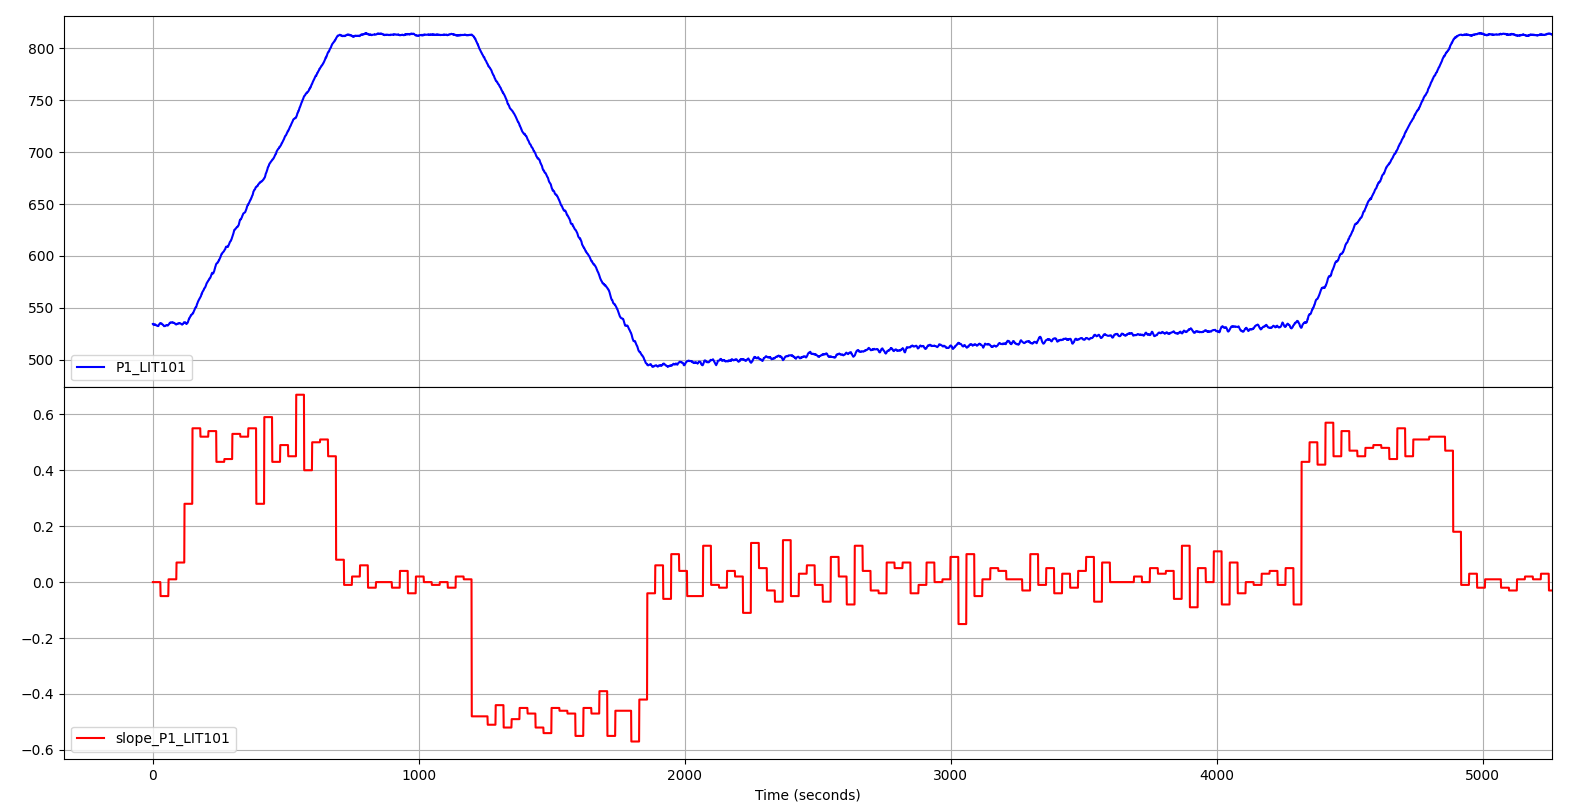
\includegraphics[width=\textwidth]{chap4/slope_nodecomp_g30_2.png}
		\caption{}
		\label{subfig:4_slope_g30_nodecomp}
	\end{subfigure}
	\hfill
	\begin{subfigure}{0.9\textwidth}
		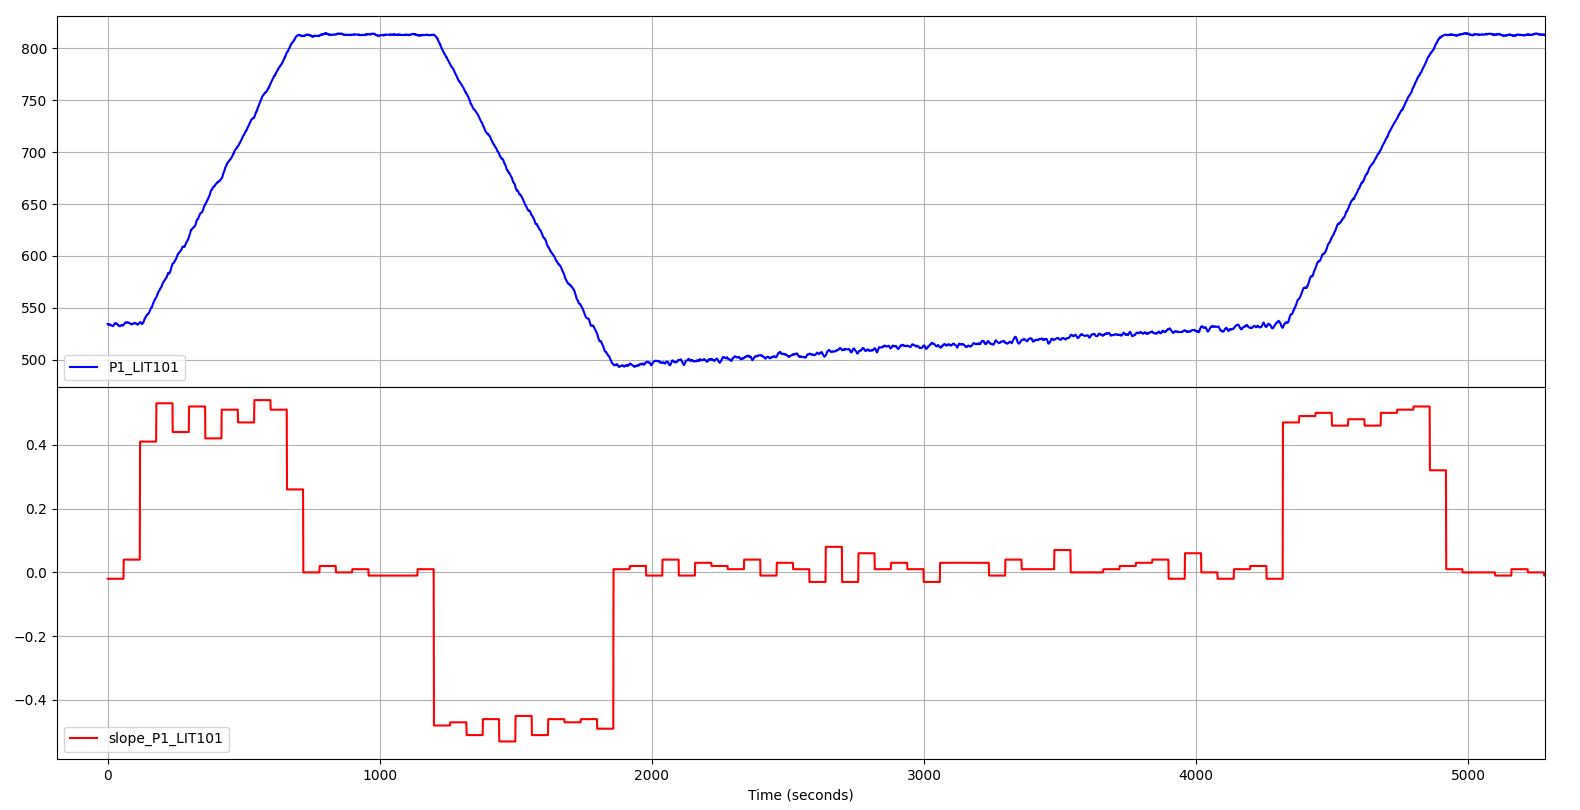
\includegraphics[width=\textwidth]{chap4/slope_nodecomp_g60_2.png}
		\caption{}
		\label{subfig:4_slope_g60_nodecomp}
	\end{subfigure}
	\begin{subfigure}{0.9\textwidth}
		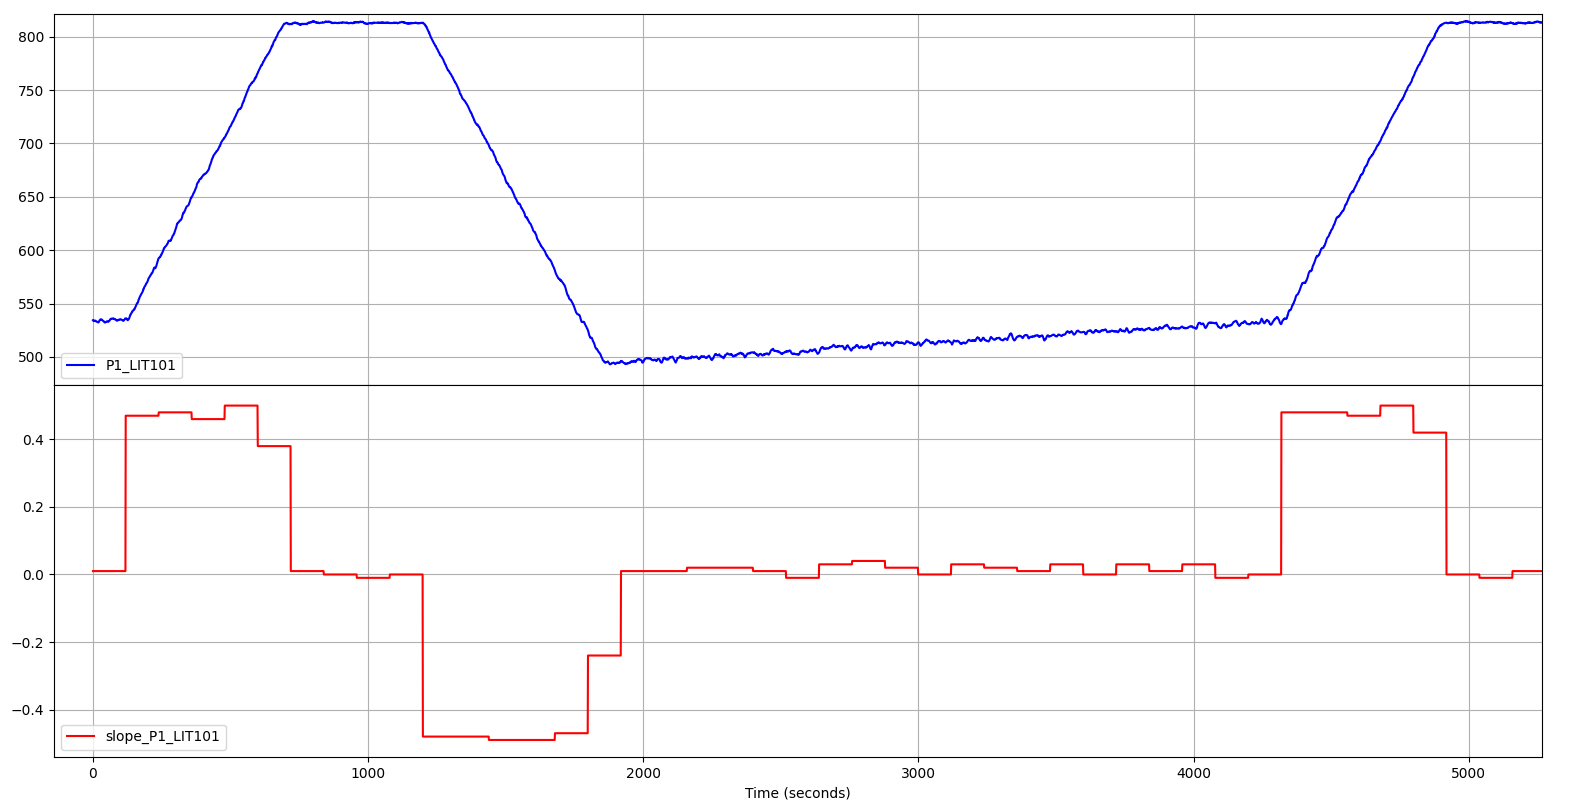
\includegraphics[width=\textwidth]{chap4/slope_nodecomp_g120_2.png}
		\caption{}
		\label{subfig:4_slope_g120_nodecomp}
	\end{subfigure}
	\caption{Slope comparison with granularity 30 (a), 60 (b) and 120 seconds (c)}
	\label{fig:4_slope_comparison}
\end{figure}

The solution to this problem involves applying techniques to reduce the "noise" in the data, aiming to achieve a more linear trend in the measurement curve. By minimizing the effects of perturbations, we can calculate slopes more accurately.\newline
There are various methods available for smoothing out noise in the data. In our framework, we focused on two commonly used approaches found in the literature: \textbf{polynomial regression} and \textbf{seasonal decomposition}.\newline \newline
\textit{Polynomial regression} is a technique that allows us to create a filter to reduce the impact of noise on the data. By fitting a polynomial function to the measurements, we can obtain a smoother curve that captures the underlying trend while minimizing the effects of perturbations.\newline
\textit{Seasonal decomposition}, specifically the part related to trending, is another method we explored. It involves decomposing the time series into different components, such as trend, seasonality, and residual. By isolating the trend component, we can obtain a cleaner representation of the underlying pattern in the data.\newline
Regarding polynomial regression, we evaluated the use of the \textbf{Savitzky-Golay filter} \cite{savgol} as a smoothing technique. For seasonal decomposition, we explored the \textbf{Seasonal-Trend decomposition using LOESS} (STL) method \cite{stl_decomp}.\newline \newline
For lacking of space we are unable to provide a detailed description of the polynomial regression and seasonal decomposition techniques in this context. We recommend referring to the bibliographical notes or relevant literature for a more comprehensive understanding of these methods: Figure \ref{fig:4_smoothing_comparison}, however, shows a quick graphical comparison of them compared with the original data. The solution adopted is the \textit{STL decomposition} method, which effectively reduces noise compared to the Savitzky-Golay filter. However, it should be noted that this method may introduce some delay in certain parts of the data, as is typically observed in similar algorithms.

\begin{figure}[H]
	\centering
	\begin{subfigure}{0.48\textwidth}
		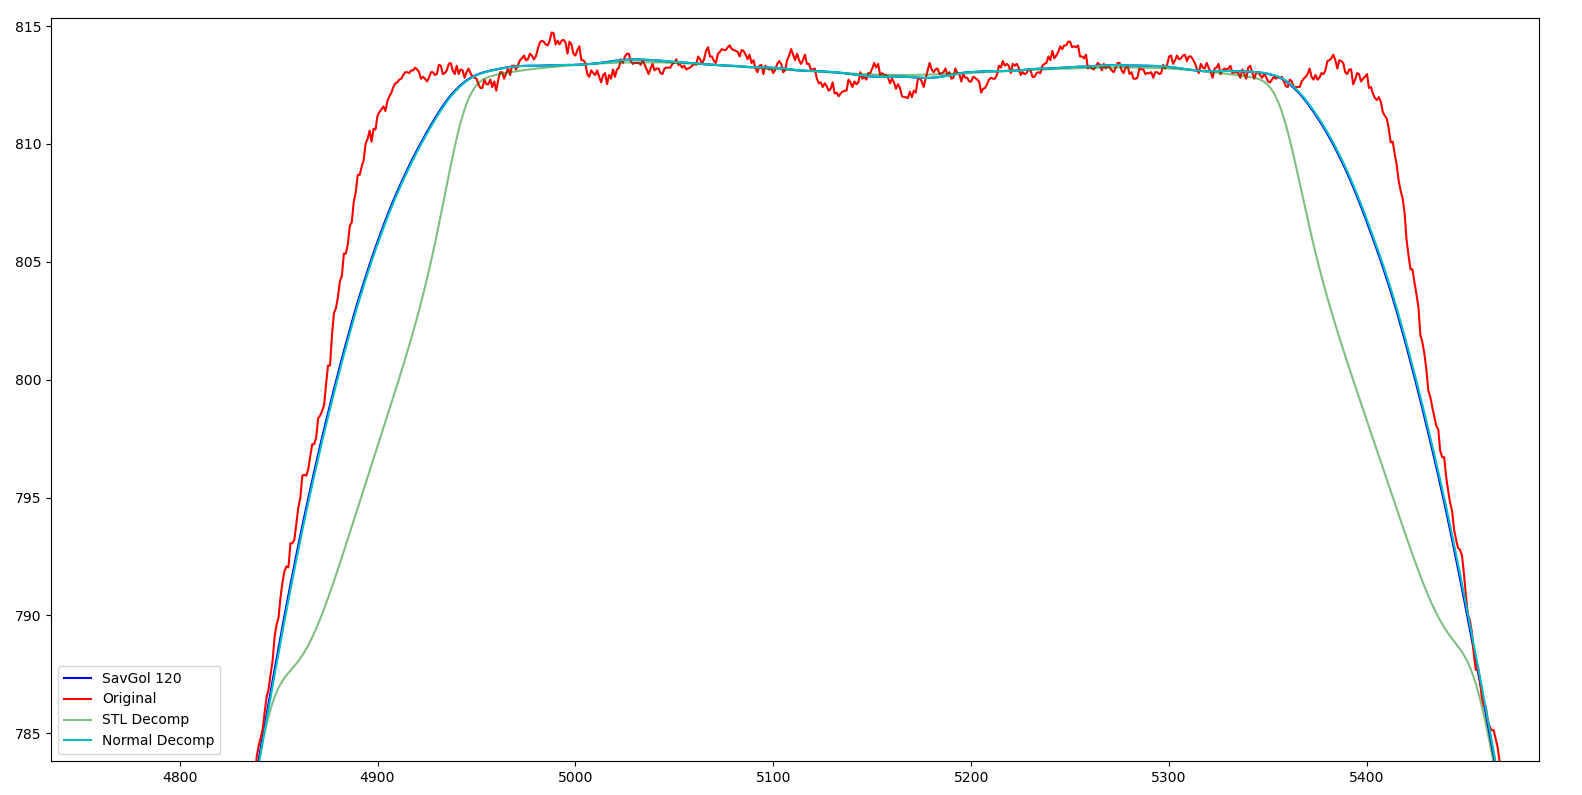
\includegraphics[width=\textwidth]{chap4/confronto_decomp_3.png}
		\caption{}
		\label{subfig:4_smoothing1}
	\end{subfigure}
	\hfill
	\begin{subfigure}{0.48\textwidth}
		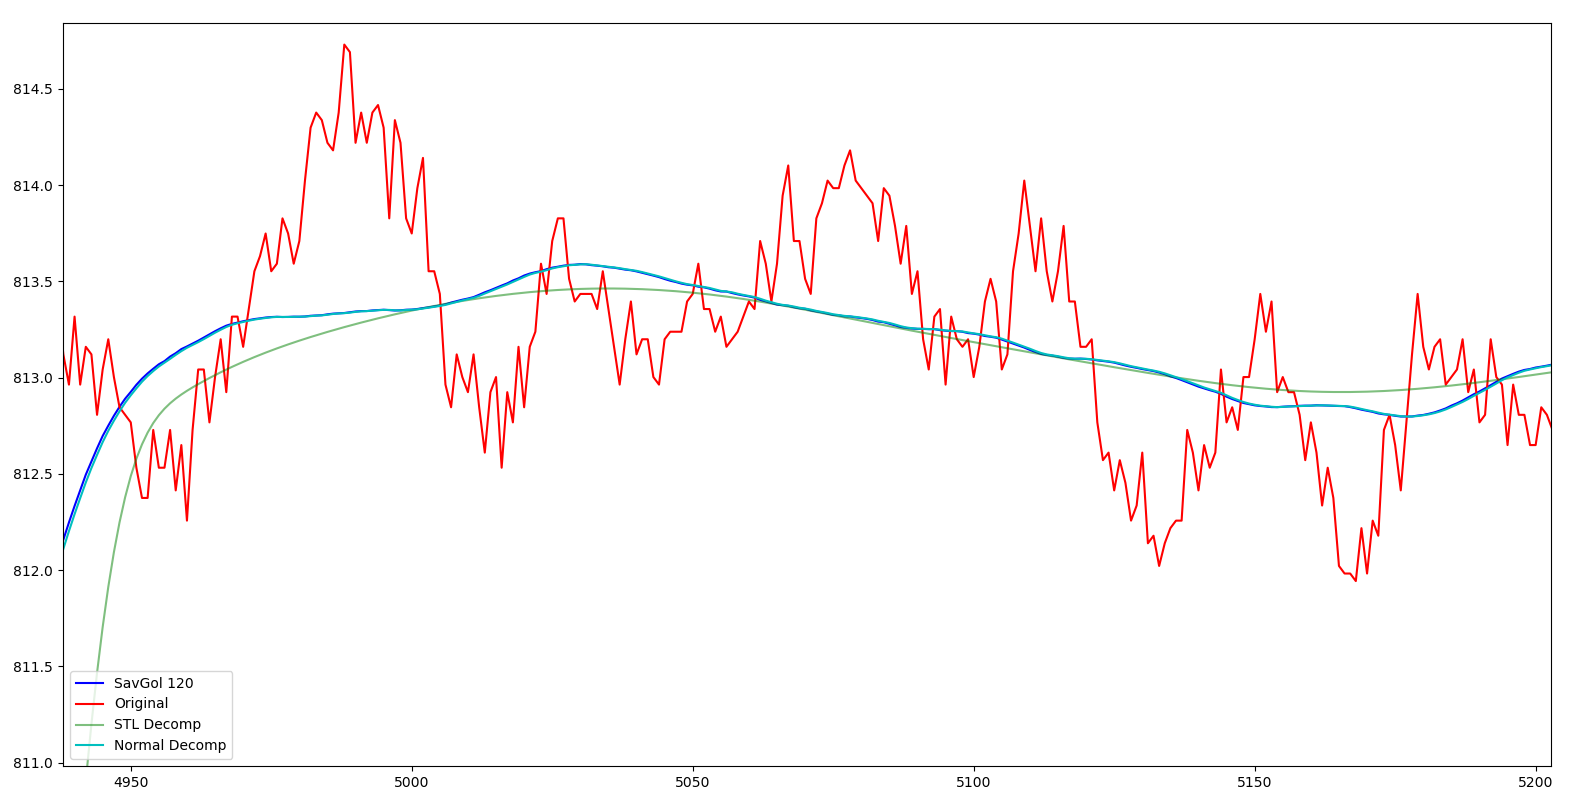
\includegraphics[width=\textwidth]{chap4/confronto_decomp_4.png}
		\caption{}
		\label{subfig:4_smoothing2}
	\end{subfigure}
	\begin{subfigure}{0.48\textwidth}
		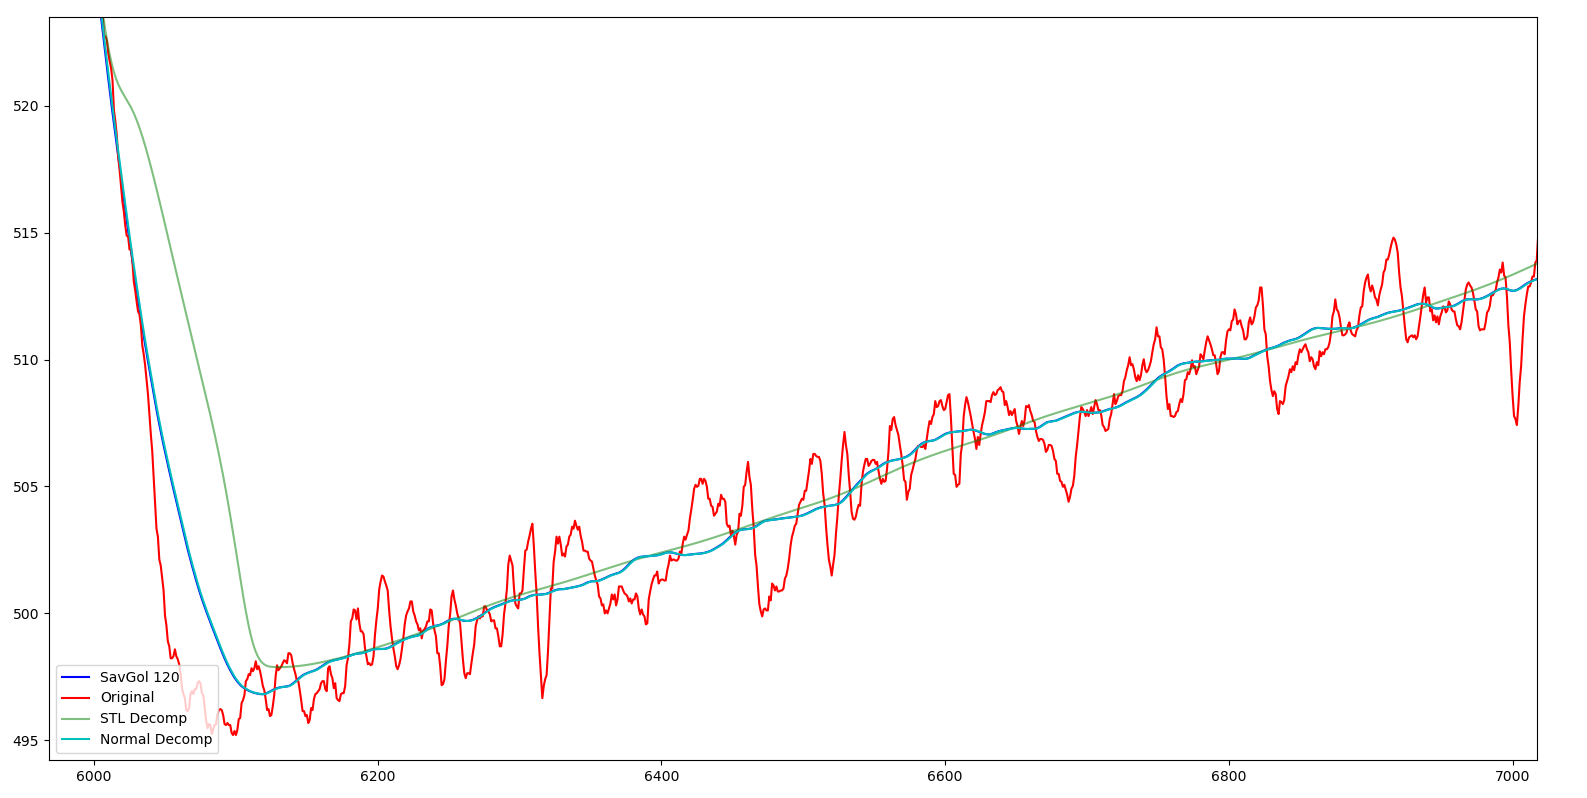
\includegraphics[width=\textwidth]{chap4/confronto_decomp_5.png}
		\caption{}
		\label{subfig:4_smoothing3}
	\end{subfigure}
	\begin{subfigure}{0.48\textwidth}
		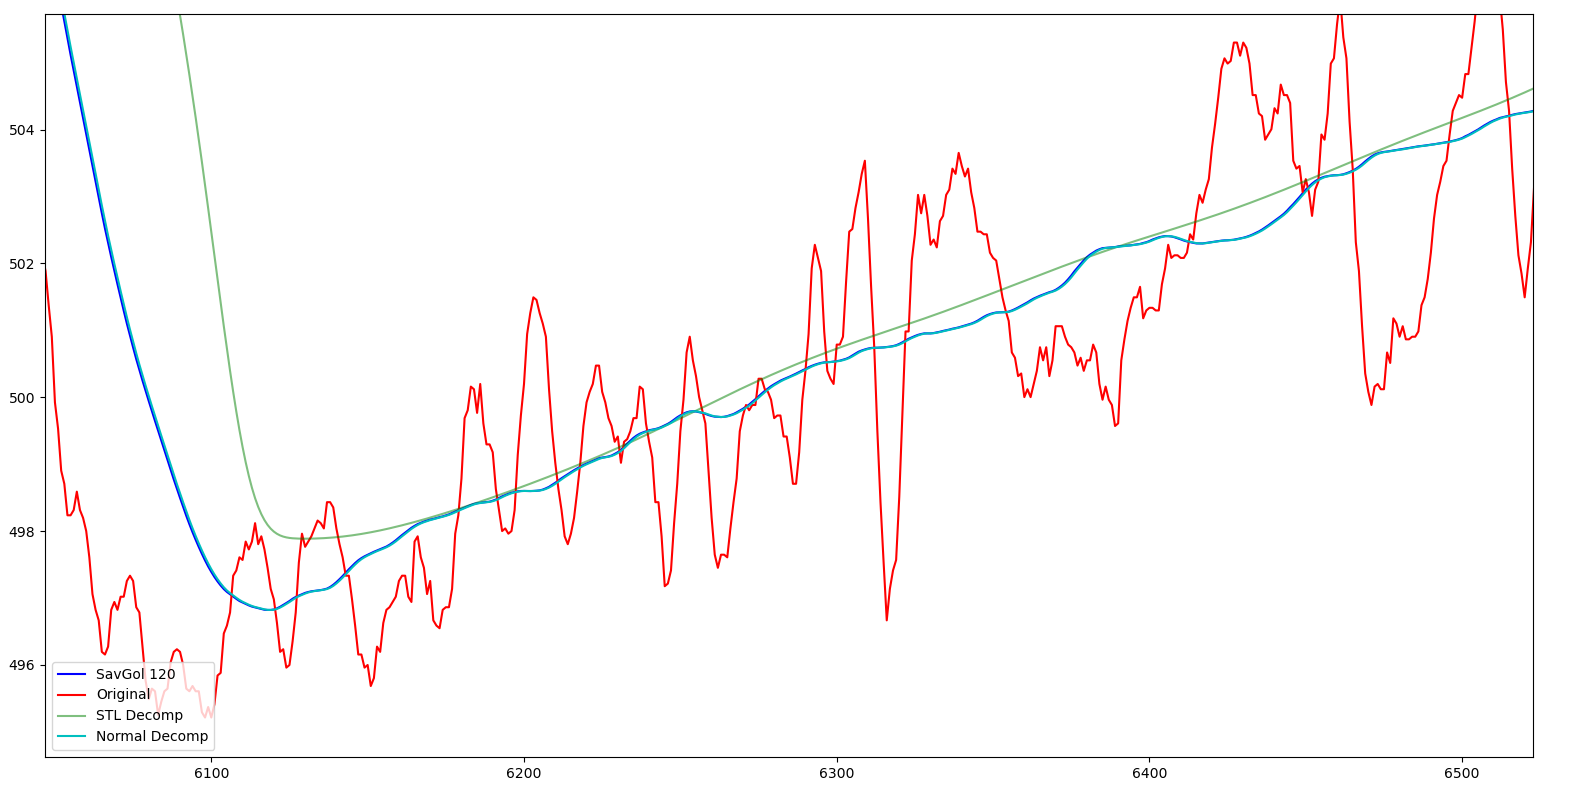
\includegraphics[width=\textwidth]{chap4/confronto_decomp_6.png}
		\caption{}
		\label{subfig:4_smoothing4}
	\end{subfigure}
	\caption{Savitzky-Golay filter (blue line) and STL decomposition (green) comparison}
	\label{fig:4_smoothing_comparison}
\end{figure}

By applying the STL decomposition, we observe a notable enhancement in slope calculation even when using a low granularity. Figure \ref{fig:4_STL_decomp_results} demonstrates that, with the same granularity as shown in Figure \ref{subfig:4_slope_g30_nodecomp}, the slope values, albeit exhibiting fluctuations, consistently align with the underlying trend of the data curve. The introduced lag resulting from the decomposition's periodicity is responsible for the observed delay.

\begin{figure}[ht]
	\centering
	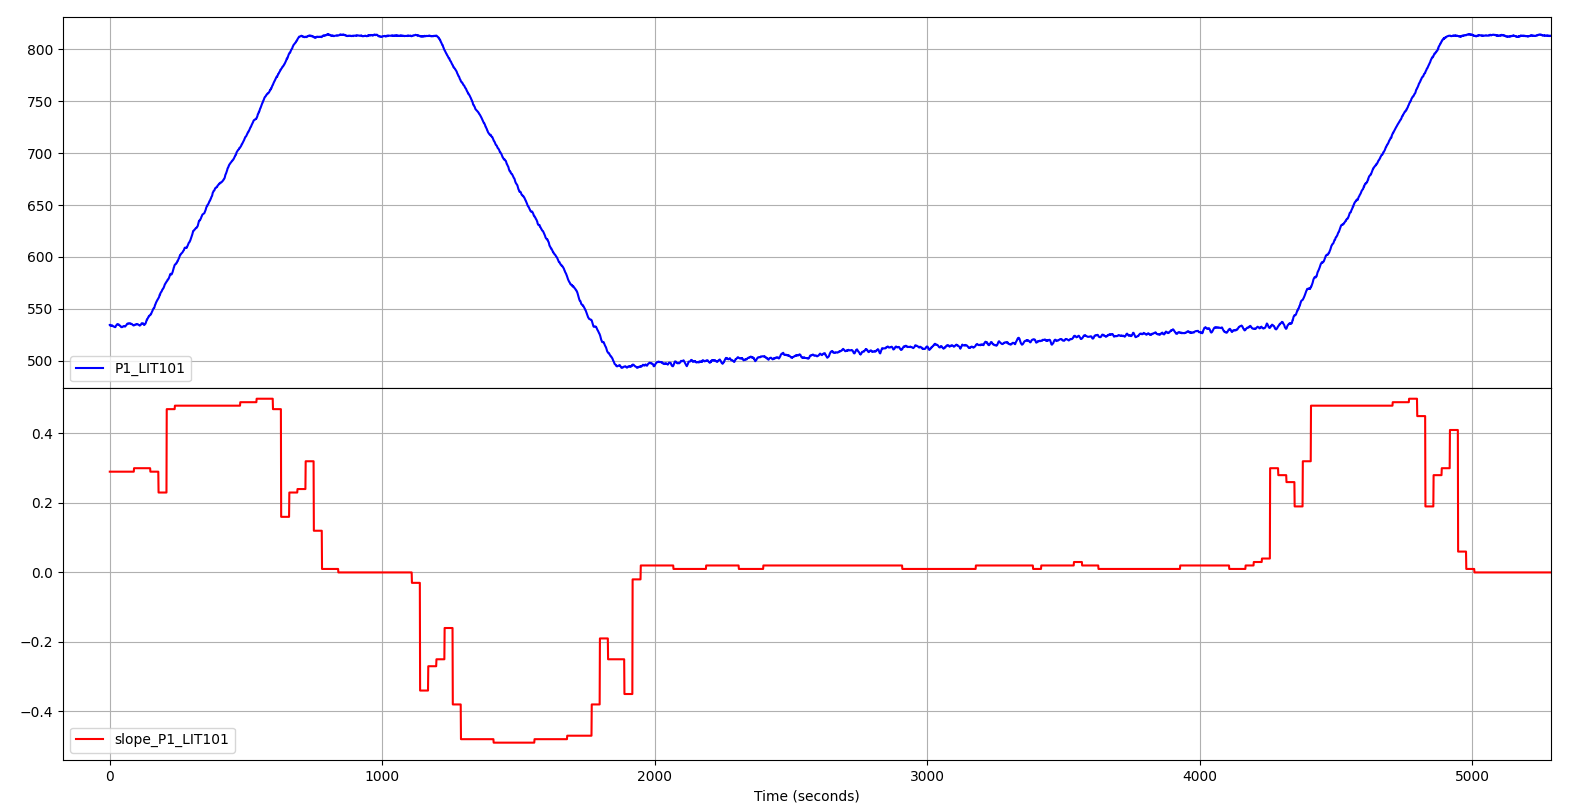
\includegraphics[scale=0.35]{chap4/slope_STL_g30_2.png}
	\caption{Slope after the application of the STL decomposition}
	\label{fig:4_STL_decomp_results}
\end{figure}
The periodicity, determining the sampling time window for decomposition and noise smoothing level, can be specified in the \texttt{trend\_period} directive of the \textit{config.ini} configuration file.\newline
The slope calculation will be applied to the data from the additional measurement trend attributes, which are defined in the \texttt{trend\_cols\_list} directive of the configuration file, rather than the original unfiltered data.

\bigskip
To ensure proper interpretation by Daikon, the decimal values representing the calculated slopes are converted into three numerical values: -1, 0, and 1. These values correspond to decreasing (if the slope is less than zero), stable (if it is equal to zero), and increasing (if it is greater than zero) trends, respectively. Figure \ref{fig:4_slope_daikon} displays the modified slopes along with the curve obtained from the STL decomposition:

\begin{figure}[ht]
	\centering
	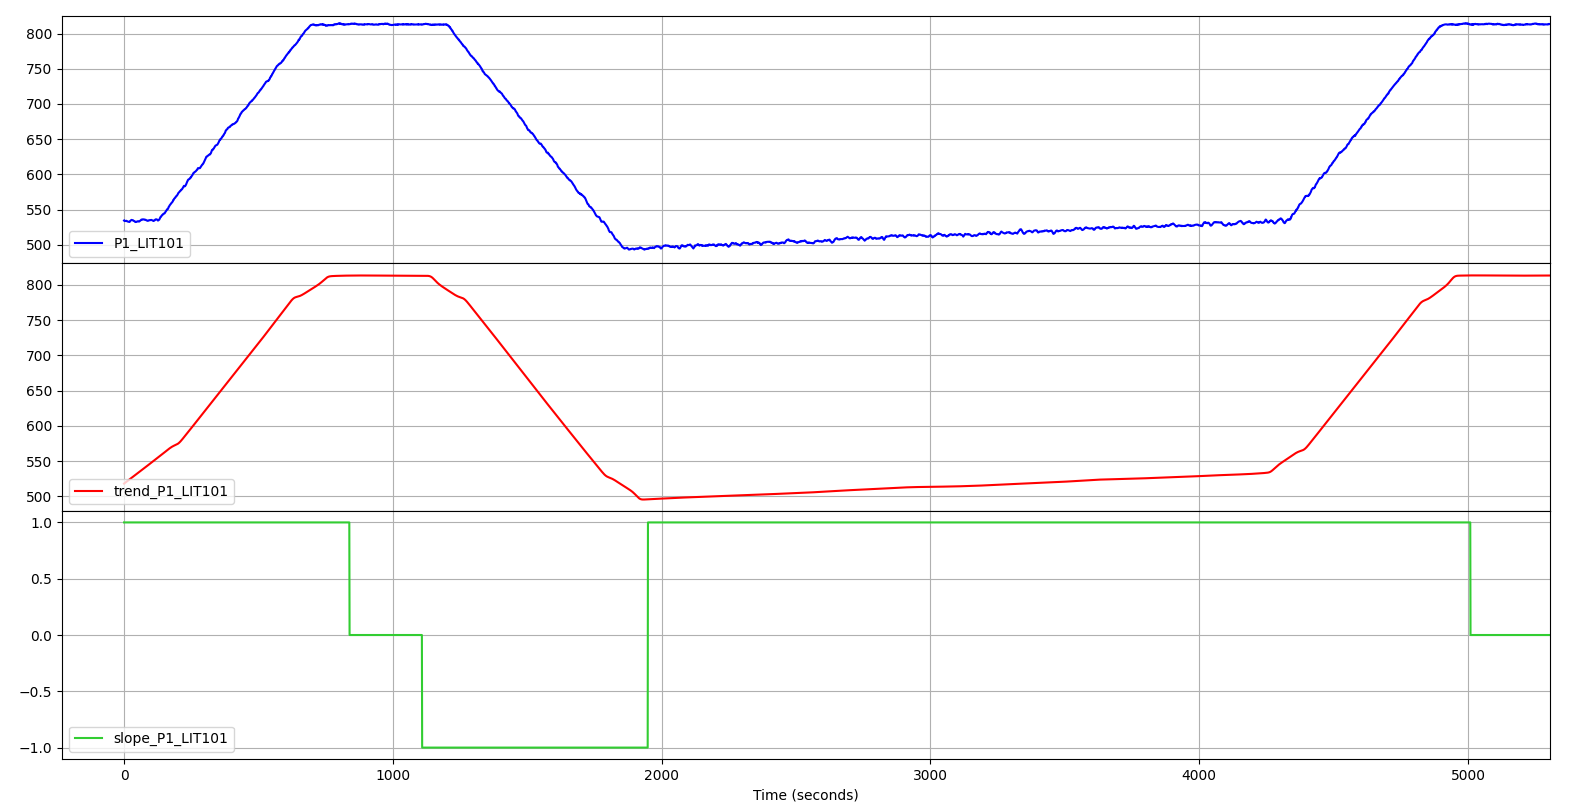
\includegraphics[scale=0.35]{chap4/slope_STL_bin_g30_2b.png}
	\caption{The new slope representation (green line) and the smoothed measurement data obtaind with the STL decomposition (red)}
	\label{fig:4_slope_daikon}
\end{figure}

\subsubsection{Datasets Merging}
\label{subsubsec:4_dataset_merging}
During this step, the datasets of the individual PLCs are merged, resulting in two separate datasets. The first dataset is enriched with additional attributes but excludes the timestamp column. This dataset is intended for inference and invariant analysis. The second dataset does not contain any additional data and is specifically used in the process mining phase.

\bigskip
By default, the enriched dataset will be saved in CSV format in the \texttt{\$(project-dir)/daikon/Daikon\_Invariants} directory. The other dataset, without additional data, will be saved in the \texttt{\$(project-dir)/process-mining/data directory}. It's worth noting that both paths can be configured in the \textit{config.ini} file. The dataset name can be specified in the \textit{config.ini} file or through the \texttt{-o} command-line option. When generating the dataset for process mining, the script will automatically add a \texttt{\_TS} suffix to the filename to indicate that it includes the timestamp. This flexibility allows the user to provide a different filename for each output, preventing overwriting of previous datasets. It enables the user to save the execution trace of the selected subsystem separately and utilize them in subsequent analysis phases.

\subsubsection{Brief Analysis of the Obtained Subsystem}
\label{subsubsec:4_brief_analysis}

After merging the datasets, the user has the option to perform an \textbf{optional analysis} of the resulting dataset to extract preliminary data. This analysis aims to gather basic information about the (sub)system and potentially refine the enrichment process. If the user chooses to proceed with the analysis, the \texttt{mergeDatasets.py} script invokes another Python script located in the \texttt{\$(project-dir)/pre-processing} directory called \texttt{system\_info.py}.\newline
Relying on an analysis based on a combination of Daikon and Pandas this script performs a quick analysis of the dataset allowing to \textbf{estimate}, albeit approximately, the \textbf{type of registers} (sensors, actuators, ...), also identifying possible maximum and minimum values of measurements and hardcoded setpoints. Furthermore, leveraging the use of the additional attribute \texttt{prev\_}, the \texttt{system\_info.py} script is capable of deriving measurement values corresponding to state changes of individual actuators. This allows for the identification of specific measurements associated with the activation or deactivation of certain actuators within the system.\newline 
Listing \ref{lst:4_brief_infos} shows an example of this brief analysis related to PLC1 of the iTrust SWaT system (for brevity, only one measurement is reported in the analysis of actuator state changes):

\begin{lstlisting}[language=bash,numbers=none,caption={Example of preliminar system analysis},label=lst:4_brief_infos]
	Do you want to perform a brief analysis of the dataset? [y/n]: y
	
	Actuators: 
	P1_MV101 [0.0, 1.0, 2.0]
	P1_P101 [1.0, 2.0]
	
	Sensors: 
	P1_FIT101 {'max_lvl': 2.7, 'min_lvl': 0.0}
	P1_LIT101 {'max_lvl': 815.1, 'min_lvl': 489.6}
	
	Hardcoded setpoints or spare actuators: 
	P1_P102 [1.0]
	
	Actuator state changes:
	       P1_LIT101  P1_MV101  prev_P1_MV101
	669     800.7170         0              2
	1850    499.0203         0              1
	4876    800.5992         0              2
	6052    498.9026         0              1
	9071    800.7170         0              2
	10260   499.1381         0              1
	13268   801.3058         0              2
	14435   498.4315         0              1
	17423   801.4628         0              2
	18603   498.1567         0              1
	
	P1_LIT101  P1_MV101  prev_P1_MV101
	677     805.0741         1              0
	4885    805.7414         1              0
	9079    805.7806         1              0
	13276   805.1133         1              0
	17432   804.4068         1              0
	
	P1_LIT101  P1_MV101  prev_P1_MV101
	1858    495.4483         2              0
	6060    497.9998         2              0
	10269   495.9586         2              0
	14443   495.8016         2              0
	18611   494.5847         2              0
	
	       P1_LIT101  P1_P101  prev_P1_P101
	118     536.0356        1             2
	4322    533.3272        1             2
	8537    542.1591        1             2
	12721   534.8581        1             2
	16883   540.5890        1             2
	
	P1_LIT101  P1_P101  prev_P1_P101
	1190    813.0031        2             1
	5395    813.0031        2             1
	9597    811.8256        2             1
	13776   812.7283        2             1
	17938   813.3171        2             1
	
	Actuator state durations:
	P1_MV101 == 0.0
	9  9  10  9  9  10  9  9  10  9
	
	P1_MV101 == 1.0
	1174  1168  1182  1160  1172
	
	P1_MV101 == 2.0
	669  3019  3012  3000  2981
	
	P1_P101 == 1.0
	1073  1074  1061  1056  1056
	
	P1_P101 == 2.0
	118  3133  3143  3125  3108
\end{lstlisting}

From these results we can draw the following conjectures: 

\begin{itemize}
	\item the \textbf{probable actuators} are \texttt{P1\_MV101} and \texttt{P1\_P101}. \texttt{P1\_MV101} has three states identified by the values 0, 1, and 2, suggesting it is a multi-state actuator. \texttt{P1\_P101} has two states identified by the values 1 and 2, indicating a binary actuator;
	
	\item there are \textbf{two probable measures}: \texttt{P1\_FIT101} and \texttt{P1\_LIT101}. \texttt{P1\_FIT101} has values ranging from 0 to 2.7, \texttt{P1\_LIT101} has values ranging from 489.6 to 815.1. Based on this information, a further conjecture can be made that \texttt{P1\_LIT101} represents a tank level measurement;
		
	\item apparently there is a probable \textbf{spare actuator}, \texttt{P1\_P102}, whose value is always 1. No related \textit{hardcoded setpoints} were found. From this information, another speculation can be made that the value 1 represents the \textbf{OFF state} for binary actuators, while the value 2 represents the \textbf{ON state};
	
	\item from the analysis of state changes we can derive some \textbf{relative setpoints}. For example, we observe that \texttt{P1\_P101} changes state from value 1 (OFF) to value 2 (ON) when the level of \texttt{P1\_LIT101} is approximately 813, and it changes from value 2 (ON) to 1 (OFF) when the level of \texttt{P1\_LIT101} is around 535. We can deduce that \texttt{P1\_P101} is responsible for emptying the tank;
	
	\item as the last information we have duration of actuator states for each cycle of the system: this information can be useful for making assumptions and conjectures about the behavior of an actuator in a specific state or, by observing the duration values of each cycle, highlighting anomalies in the system.\newline
	In the specific case, the very short duration of \texttt{P1\_MV101} in state 0 is observable: since we are unable, at this preliminary stage, to make assumptions about this, we will try to understand the behavior of the system in this actuator state in the next stages of the analysis
\end{itemize}

The information obtained here can be used, as mentioned above, to refine the enrichment of the dataset by setting directives in the \texttt{[DATASET]} section of the \textit{config.ini} file, should this be empty or only partially set, or to make the first conjectures about the system, as we have just seen.

\bigskip
The \texttt{system\_info.py} file can also run in standalone mode if needed: it takes as command-line arguments the dataset to be analyzed, a list of actuators, and a list of sensors. For analysis related to state changes, the dataset must mandatorily be of the enriched type.

\subsection{Phase 2: Graphs and Statistical Analysis}
\label{subsec:4_improve_graphs}

The new \textit{graph analysis} arises from the need to give the user an overview of the (sub)system obtained in the previous pre-processing phase, identifying more easily the typology of the registers and grasping more effectively the relationships and the dynamics that may exist between the registers controlled by one or more PLCs, confirming the initial conjectures if the brief analysis described in the previous section has been performed, or making new ones thanks to the visual graph support. 

\bigskip
In Ceccato et al.'s framework, as mentioned in Section \ref{subsec:3_ceccato_limitations}, it was only possible to view the chart of one register at a time. While this allowed for the identification or hypothesis of the register type, it made it challenging to establish relationships with other components of the system and derive conjectures about their behavior. To address this limitation, there was a need for a new tool that could provide more information in a more accessible manner.

\bigskip
Initially, we considered adopting an approach similar to Figure \ref{fig:graph_analysis_prop3}, where all the graphs are displayed within a single plot. However, we soon realized that this solution was not feasible and could not be adopted. Figure \ref{fig:4_plot_comparison_1} helps to understand why.  

\begin{figure}[H]
	\centering
	\begin{subfigure}{0.48\textwidth}
		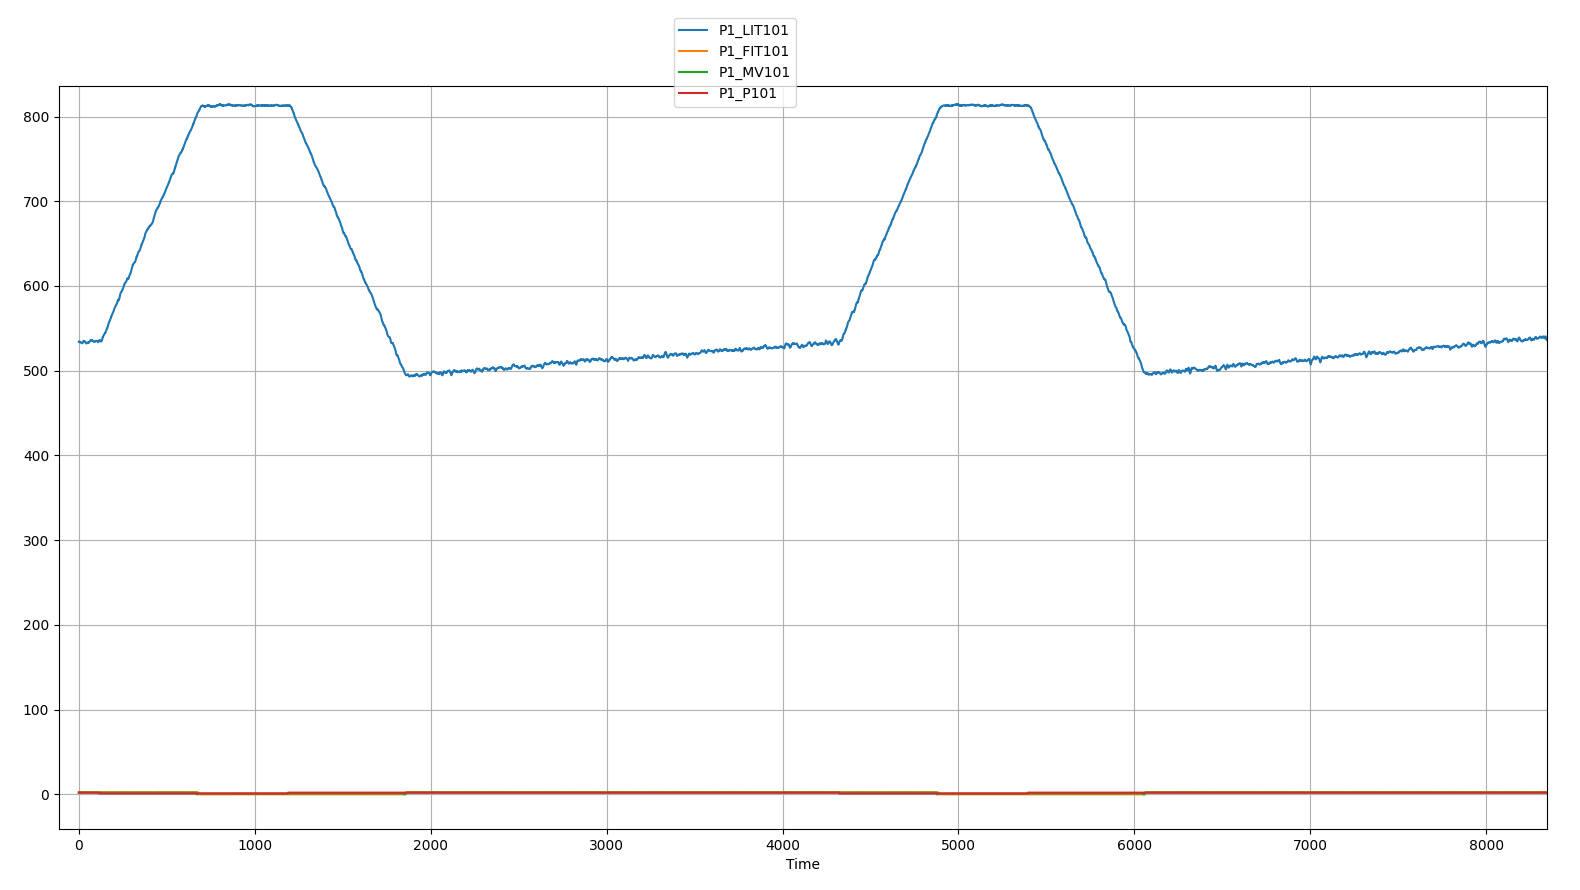
\includegraphics[width=\textwidth]{chap4/wrong_plot_1.png}
		\caption{}
		\label{subfig:4_wrong_plot}
	\end{subfigure}
	\hfill
	\begin{subfigure}{0.48\textwidth}
		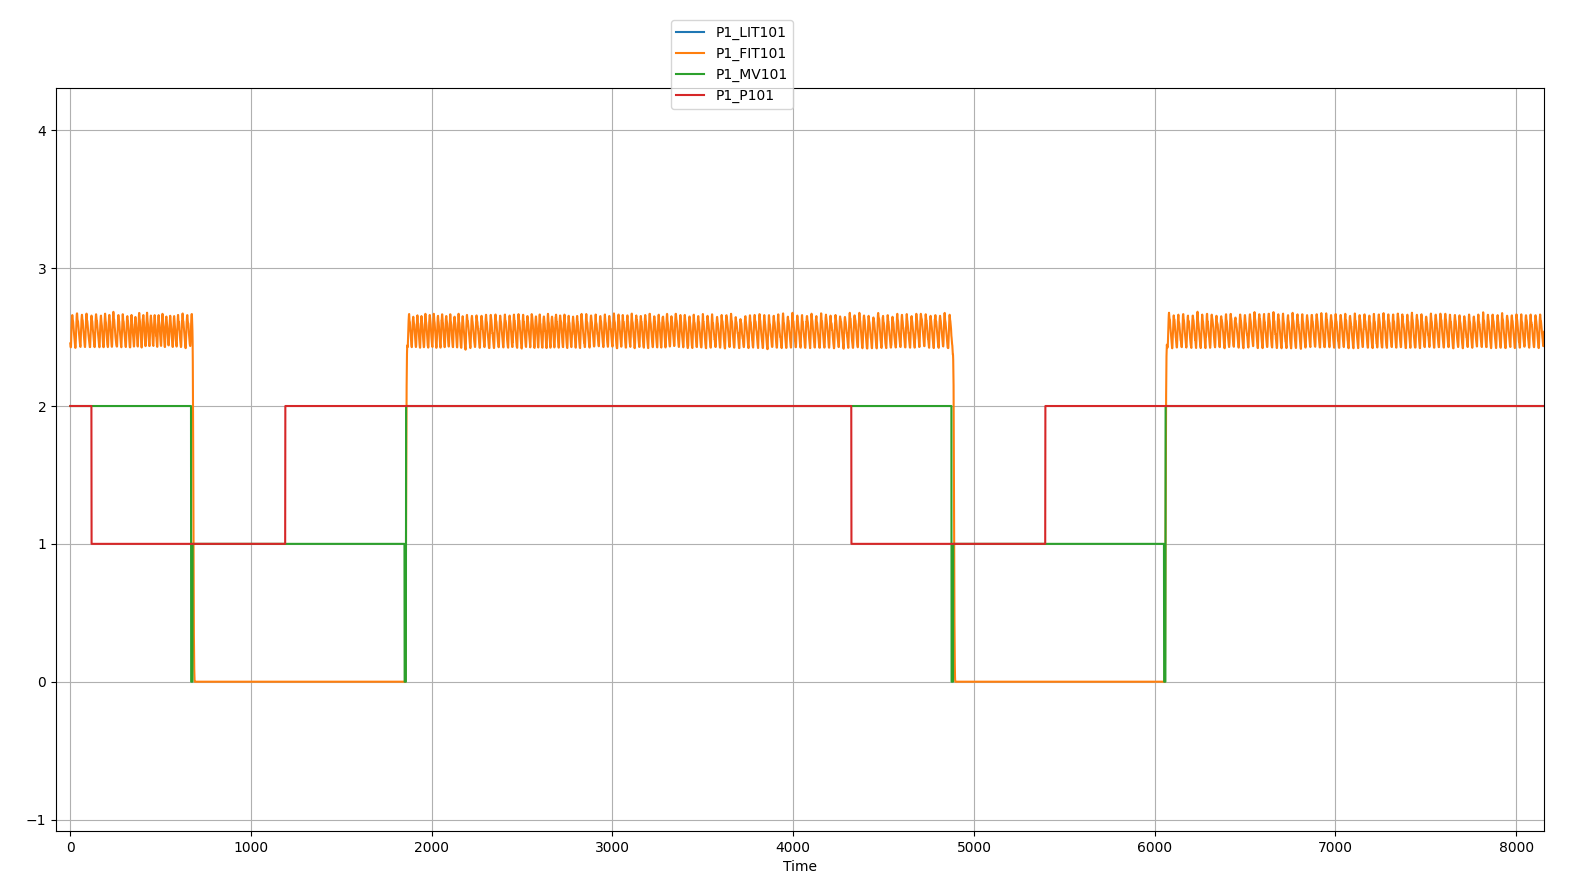
\includegraphics[width=\textwidth]{chap4/wrong_plot_2.png}
		\caption{}
		\label{subfig:4_wrong_plot_zoom}
	\end{subfigure}
	\caption{Plotting registers on the same y-axis}
	\label{fig:4_plot_comparison_1}
\end{figure}
Figure \ref{subfig:4_wrong_plot} highlights the main issue with this approach, which is the use of the same y-axis for all the charts, representing the values of individual registers. When the range between register values is wide, it can result in some charts appearing as a single flat line or becoming indistinguishable, making them difficult to read. Additionally, as shown in Figure \ref{subfig:4_wrong_plot_zoom}, when registers have similar values, the graphs can become confusing and harder to interpret.

\bigskip
The solution to this issue is simple and effective: the use of \textbf{subplots}. Basically, each register corresponds to a subplot of the graph that shares the time axis (the x-axis) with the other subplots, but keeps the y-axis of the values of each register independent. This maintains the readability and comprehensibility of the charts, while simultaneously being able to immediately grasp the relationships between them. In addition, by sharing the time axis, it is possible to zoom in on a particular area of one of the charts and automatically the other ones will be zoomed in as well, thus not losing any information and no connection between registers. Figure \ref{fig:4_graph_analysis} illustrates more clearly what has just been explained: the charts refer to the PLC1 registers of the iTrust SWaT system.

\begin{figure}[H]
	\centering
	\begin{subfigure}{0.9\textwidth}
		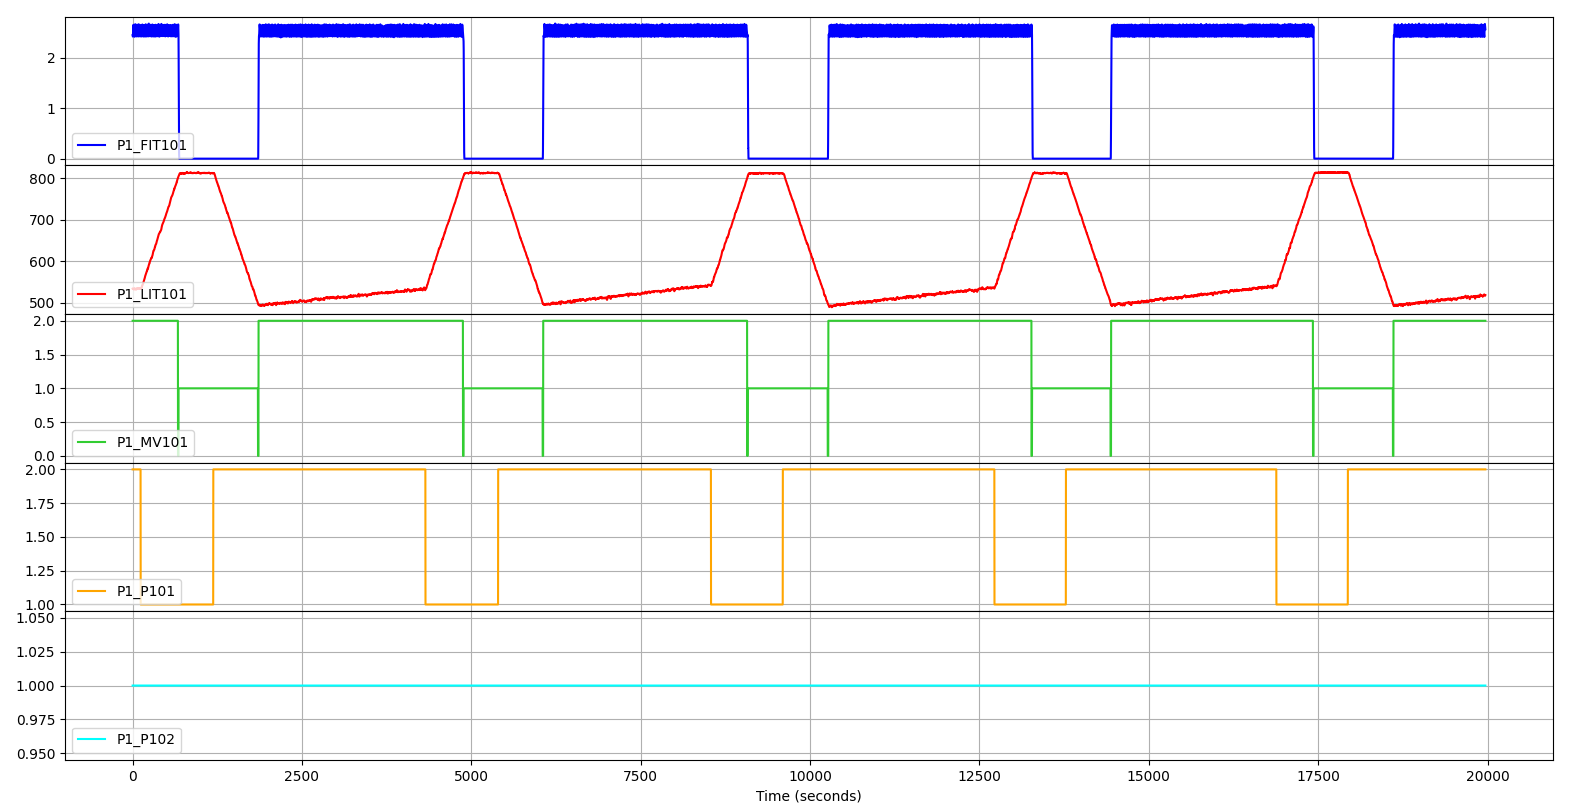
\includegraphics[width=\textwidth]{chap4/graph_analysis_plot_1.png}
		\caption{Example of plotting charts of a PLC registers using subplots}
		\label{subfig:4_graph_analysis_1}
	\end{subfigure}
	\hfill
	\begin{subfigure}{0.9\textwidth}
		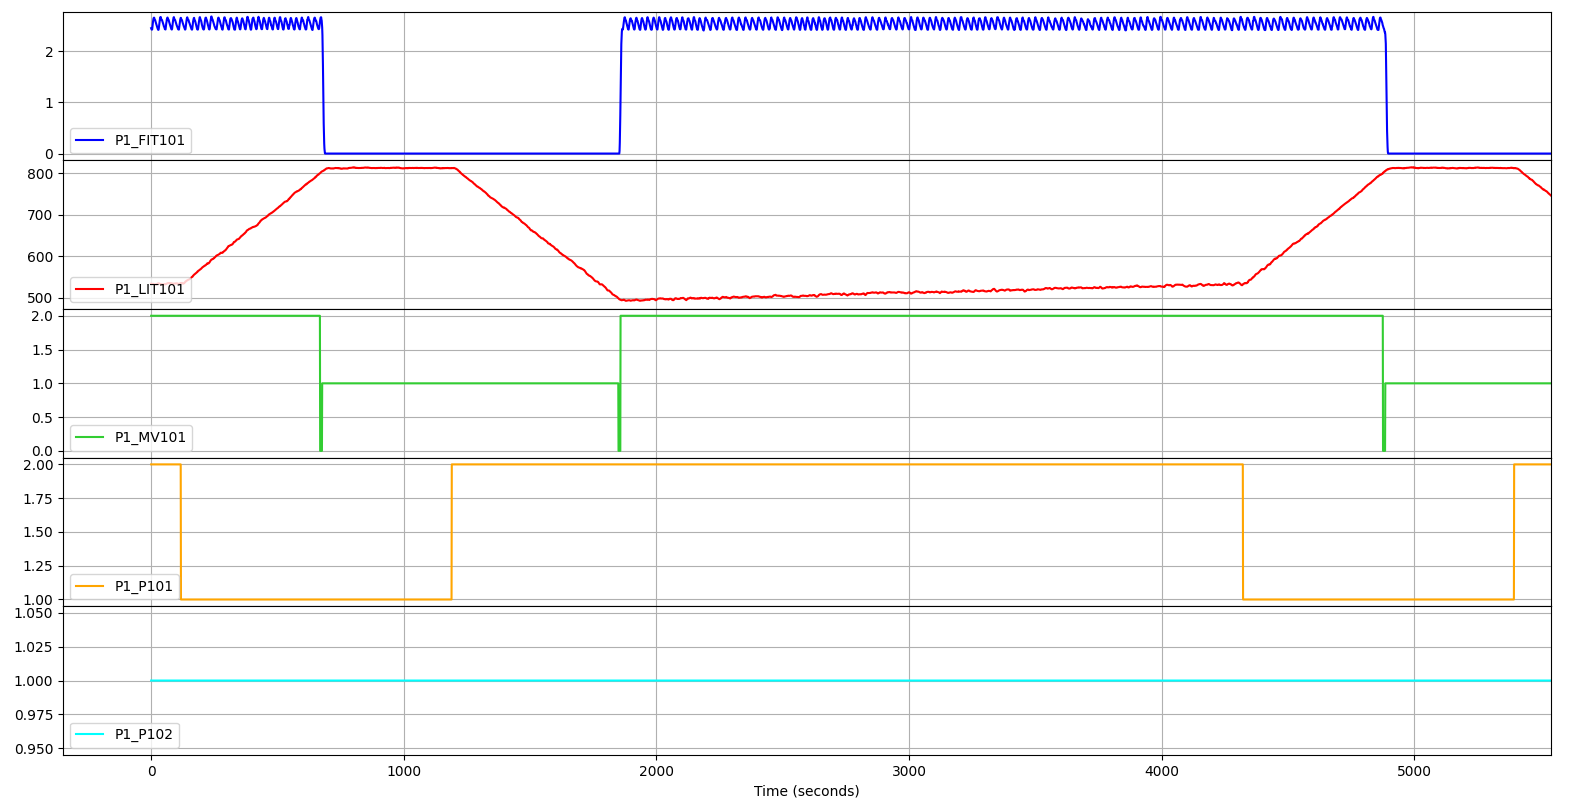
\includegraphics[width=\textwidth]{chap4/graph_analysis_plot_2.png}
		\caption{Zooming on a particular zone of the charts}
		\label{subfig:4_graph_analysis_2}
	\end{subfigure}
	\caption{Example of the new graph analysis}
	\label{fig:4_graph_analysis}
\end{figure}

\bigskip
To demonstrate the behavior and effectiveness of the new graph analysis process, we observe in particular, Figure \ref{subfig:4_graph_analysis_2}: we can already have some validation on the conjectures made in the brief analysis from the previous step:

\begin{itemize}
	\item the chart of \texttt{P1\_FIT101} seems to confirm that this register can be associated with a \textbf{measurement}; moreover, we can see that the trend of this register is closely related to the periods in which \texttt{P1\_LIT101} has an increasing trend and to the evolution of \texttt{P1\_MV101}. Its values, between about 0 and 2.5, are too narrow to say that this register represents the tank, and the general trend also leads in that direction: we can therefore assume that it is a \textbf{pressure or flow sensor}
	
	\item \texttt{P1\_LIT101}, because of the above, would therefore seem to \textbf{represent a tank}, as already assumed in the brief analysis
	
	\item \texttt{P1\_MV101} assumes value 2 at the beginning of the ascending trend of \texttt{P1\_LIT101}, while it has value 1 in correspondence with the \textit{plateau} that is seen when the measurement is about 800 and when the trend of it is descending. Thus, we can have a confirmation of the initial conjecture: 1 represents the OFF state of the sensor, 2 the ON state, and \texttt{P1\_MV101} is the \textbf{actuator responsible for the rising level} of \texttt{P1\_LIT101}
	
	\item \texttt in the brief analysis we observed the short duration of \texttt{P1\_MV101} in state 0, but we were not able to speculate on the reason for this. Graph analysis shows that {P1\_MV101} switches and stays in the 0 state acting as a kind of "transient" between states 1 and 2. It can be assumed that that is the period of time it actually takes for the actuator to change state
	
	\item \texttt{P1\_P101} assumes value 2 at the beginning of the descending trend of \texttt{P1\_LIT101}, after the \textit{plateu}, and returns to value 1 at the change of slope of the (likely) tank increase: taken by itself this fact is not very clear, so it needs to be compared with \texttt{P1\_LIT101} and \texttt{P1\_MV101} to understand its behavior: it can be seen that when \texttt{P1\_101} and \texttt{P1\_MV101} are in state 1 the water level remains stable, whereas, when \texttt{P1\_P101} changes to state 2 the level of the measurement drops rapidly; when \texttt{P1\_MV101} then also returns to state 2, the level of the measurement slowly starts rising again and then has a sudden rise at the change of state of \texttt{P1\_P101} from 2 to 1. We can therefore infer that \texttt{P1\_P101} is the \textbf{actuator responsible for emptying} the (presumed) tank: state 1 represents the OFF state, while state 2 represents the ON state
	
	\item \texttt{P1\_P102} seems to play no role in the system, since its state remains at 1 all the time. It seems improbable that it could be a relative setpoint, so it can be assumed, according to the brief analysis, that it may be a \textbf{spare actuator}
\end{itemize}

\bigskip
As you have probably already noticed, the vast majority of the graphs shown in the previous sections and chapters were generated precisely using the new graph analysis script.\newline
The script that performs the new graph analysis is \texttt{runChartsSubPlots.py}, located in the \texttt{\$(project-dir)/statistical-graphs} directory, which is written in Python and makes use, like the previous one, of the \textit{matplotlib} libraries to generate the graph plots.\newline
The script accepts the following command-line parameters:

\begin{itemize}
	\item \textbf{-f} or \textbf{{-}{-}filename}: specifies the dataset, in CSV format, from which to read the data. The dataset must be located within the directory containing the enriched datasets for the invariant analysis phase. If subsequent parameters are not specified, the script will show all registers in the dataset, except for additional attributes
	
	\item \textbf{-r} or \textbf{{-}{-}registers}: specifies one or more specific registers to be displayed
	
	\item \textbf{-a} or \textbf{{-}{-}addregisters}: adds one or more registers to the default visualization. This option is useful in case an additional attribute such as slope is to be analyzed
	
	\item \textbf{-e} or \textbf{{-}{-}excluderegisters}: excludes one or more specific registers from the default visualization. This option is useful to avoid displaying hardcoded setpoints or spare registers
\end{itemize}
This script, like the previous ones, is designed to provide the maximum flexibility and ease of use for the user, combined with greater power and effectiveness in deriving useful information about the analyzed system.

\paragraph{Statistical Analysis} A quick mention of the statistical analysis part: after careful evaluation, I decided \textbf{not to include this aspect} of the previous tool within the framework, because I saw no real practical use for it. The actual statistical information can be easily integrated into the brief analysis immediately following the pre-processing phase, while the histogram has relative utility and, in my opinion, is outdated by the new graph analysis I implemented. \newline
However, the Python \texttt{histPlots\_Stats.py} script remains in the directory, essentially unchanged from the one developed by Ceccato et al., in case future use is needed. 

\subsection{Phase 3: Invariant Inference and Analysis}
\label{subsec:4_improve_invariants}
The phase of invariant inference and analysis has undergone a redesign and improvement to offer the user a more comprehensive and effortless approach to identify invariants. This has been achieved through the application of new criteria to analyze and reorganize the Daikon analysis results. The outcome of this is a more compact presentation of information that highlights the possible relationships among invariants.\newline
The new design not only enables the identification of undiscovered aspects of the system behavior but also confirms the hypotheses made during the earlier stages of analysis. This step is now semi-automated, unlike before, and allows for the analysis of invariants on individual actuator states and their combinations.
\vfill

\subsubsection{Revised Daikon Output}
\label{subsub:4_new_daikon_output}
To streamline the process of identifying invariants quickly and efficiently, it is necessary to revise the output generated by standard Daikon analysis. The goal is to create a more compact and readable format for the output.
\newline \newline
The current Daikon results consist of three sections:

\begin{enumerate}
	\item the first section containing generic invariants, i.e., valid regardless of whether a condition is specified for the analysis
	
	\item the second section containing invariants obtained by specifying a condition for the analysis in the \textit{.spinfo} file 
	
	\item a third section containing the invariants that are obtained from the negations of the condition possibly specified in the .spinfo file
\end{enumerate}

In each section only a single invariant per row is shown, without relating it in any way to the others: this makes it difficult to identify significant invariants and any invariant chains that might provide much more information about the behavior of the system than the single invariant.\newline
A brief example of the structure and format of this output related to \texttt{PLC1} of the iTrust SWaT system is shown in Listing \ref{lst:4_daikon_output_plc1}, where a condition was specified on the measurement \texttt{P1\_LIT101} and on actuator \texttt{P1\_MV101}: % sono 61 righe effettive di invarianti - 48 generiche, 10 condizionali, 1 negata

\begin{lstlisting}[language=bash,numbers=none,caption={Standard Daikon output for \texttt{PLC1} of the iTrust SWaT system},label=lst:4_daikon_output_plc1]
	aprogram.point:::POINT
	P1_P102 == prev_P1_P102
	P1_FIT101 >= 0.0
	P1_MV101 one of { 0.0, 1.0, 2.0 }
	P1_P101 one of { 1.0, 2.0 }
	P1_P102 == 1.0
	max_P1_LIT101 == 816.0
	min_P1_LIT101 == 489.0
	slope_P1_LIT101 one of { -1.0, 0.0, 1.0 }
	[...]
	P1_LIT101 > P1_MV101
	P1_LIT101 > P1_P101
	P1_LIT101 > P1_P102
	P1_LIT101 < max_P1_LIT101
	P1_LIT101 > min_P1_LIT101
	[...]
	P1_MV101 < min_P1_LIT101
	P1_MV101 < trend_P1_LIT101
	P1_P101 >= P1_P102
	P1_P101 < max_P1_LIT101
	[...]
  ===============================================
	aprogram.point:::POINT;condition="P1_MV101 == 2.0 && P1_LIT101 < max_P1_LIT101 - 16 && P1_LIT101 > min_P1_LIT101 + 15"
	P1_MV101 == prev_P1_MV101
	P1_P102 == slope_P1_LIT101
	P1_MV101 == 2.0
	P1_FIT101 > P1_MV101
	P1_FIT101 > P1_P101
	P1_FIT101 > P1_P102
	P1_FIT101 > prev_P1_P101
	P1_MV101 >= P1_P101
	P1_MV101 >= prev_P1_P101
	P1_P101 <= prev_P1_P101
  ===============================================
	aprogram.point:::POINT;condition="not(P1_MV101 == 2.0 && P1_LIT101 < max_P1_LIT101 - 16 && P1_LIT101 > min_P1_LIT101 + 15)"
	P1_P101 >= prev_P1_P101
	Exiting Daikon.
\end{lstlisting}

In the framework I am presenting, this output is reduced to two sections, the general one and the elated to the user-specified condition, eliminating the one related to the negated condition because it is not useful in this context and a source of potential misinterpretation; moreover, the relationships between invariants will be highlighted instead by using \textbf{transitive closures}: transitive closure of a relation $R$ is another relation, typically denoted $R^{+}$ that adds to $R$ all those elements that, while not necessarily related directly to each other, can be reached by a \textit{chain} of elements related to each other. In other words, the transitive closure of $R$ is the smallest (in set theory sense) transitive relation $R$ such that $R$ $\subset$ $R^{+}$ \cite{transitive_closures}. 

\bigskip
To implement the transitive closure of the invariants generated by Daikon, I first divided the invariants in each section by type according to their equivalence relation, not considering all those invariants that refer to additional attributes except for the slope, and for each of them I generated a \textbf{graph} using the NetworkX libraries, connecting with an arc the registers (represented by nodes) that have a common endpoint in the invariant through the transitive property. To reconstruct the individual invariant chains, then, I used a simple \textit{Depth-first Search} (DFS) on each of the graphs, thus obtaining the desired outcome. Figure \ref{fig:4_transitive_closure_graphs} shows some examples of these graphs:

\begin{figure}[H]
	\centering
	\begin{subfigure}{0.48\textwidth}
		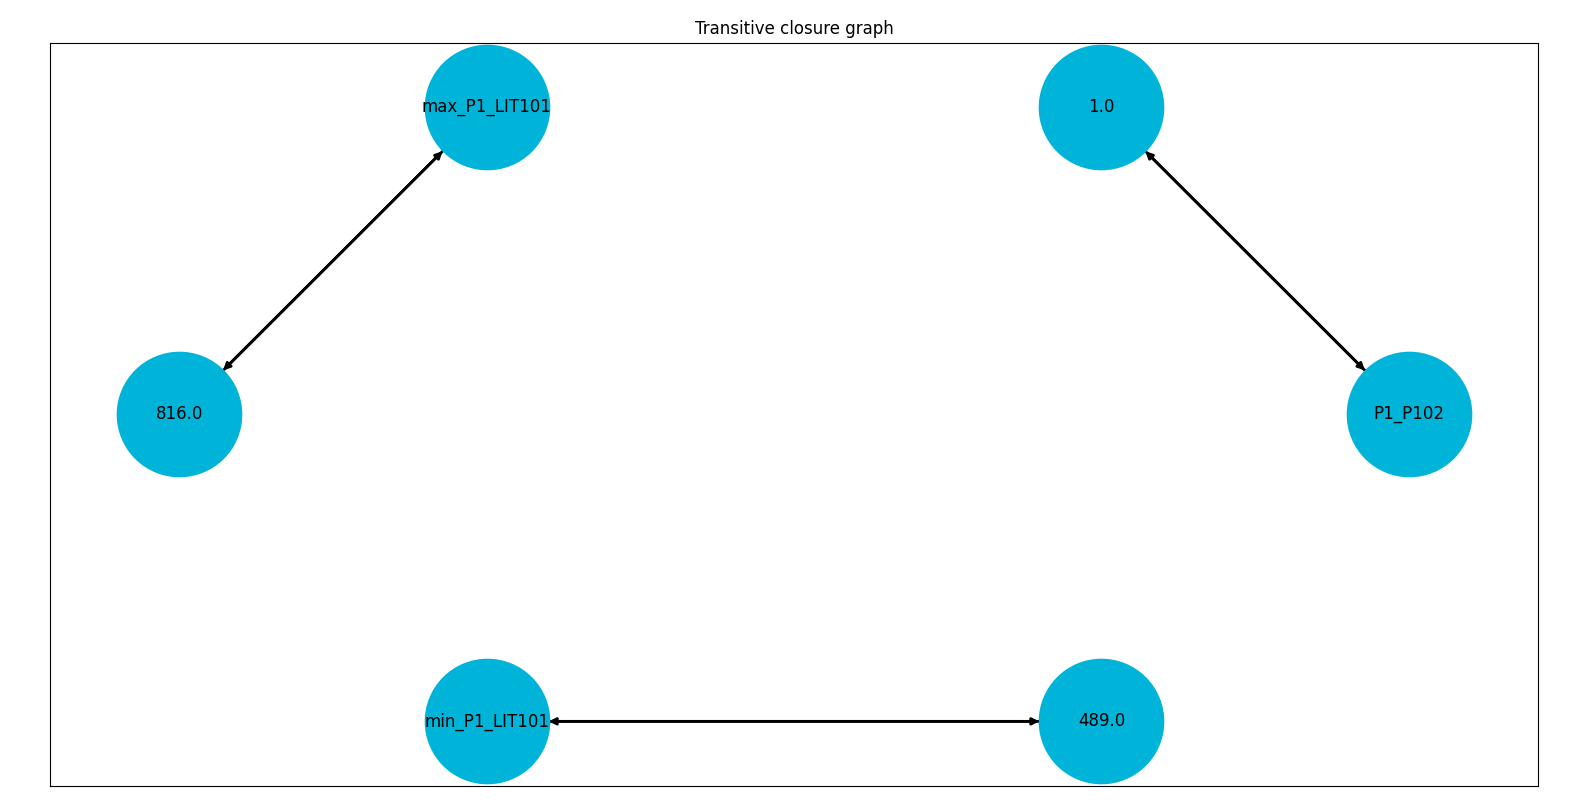
\includegraphics[width=\textwidth]{chap4/transitive_closure_eq.png}
		\caption{Transitive closure graph for "=="}
		\label{subfig:4_graph_eq}
	\end{subfigure}
	\hfill
	\begin{subfigure}{0.48\textwidth}
		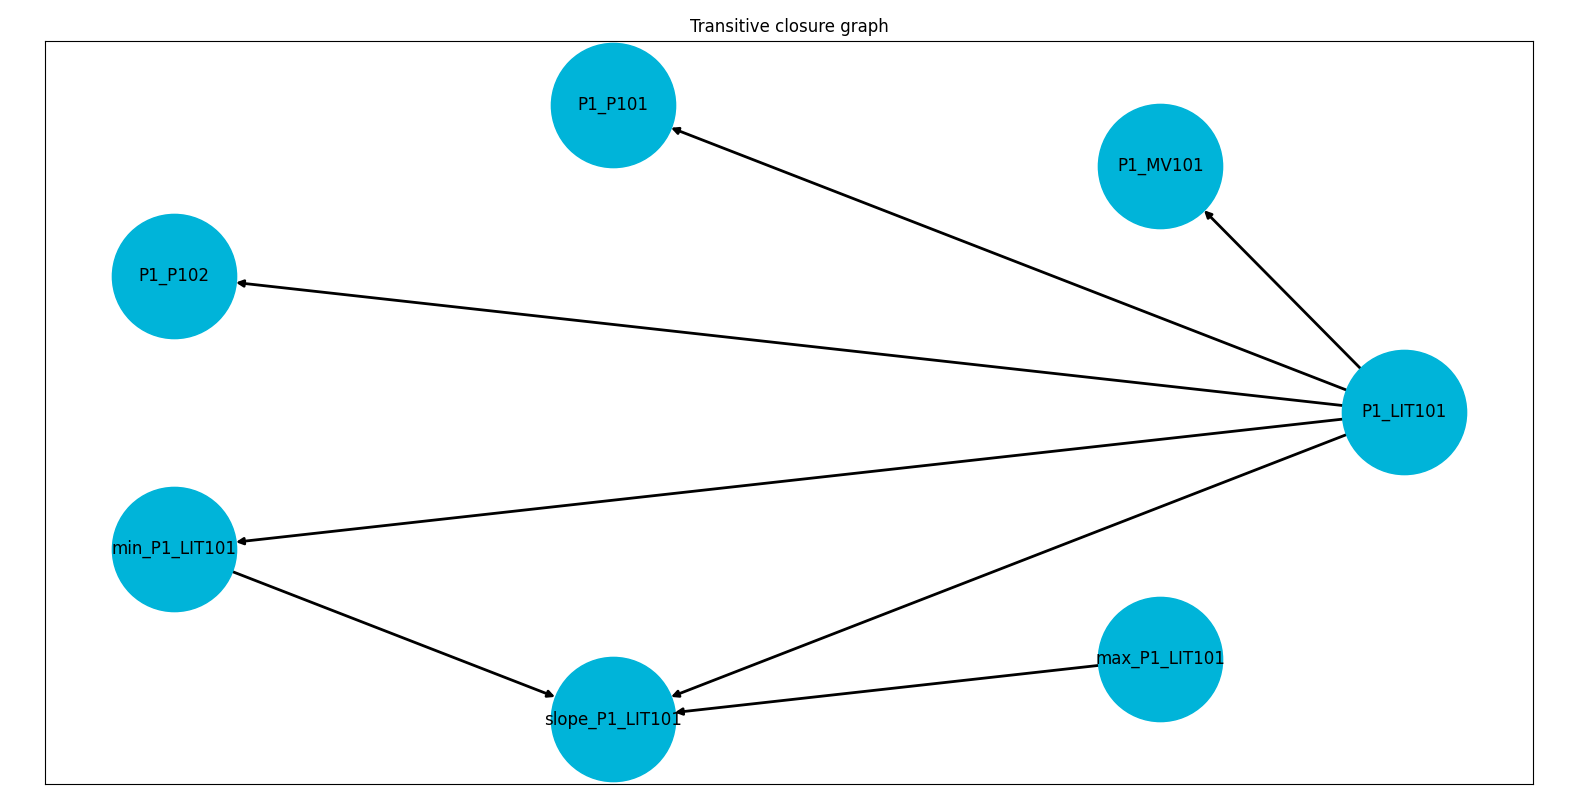
\includegraphics[width=\textwidth]{chap4/transitive_closure_gt.png}
		\caption{Transitive closure graph for ">"}
		\label{subfig:4_graph_gt}
	\end{subfigure}
	\begin{subfigure}{0.48\textwidth}
		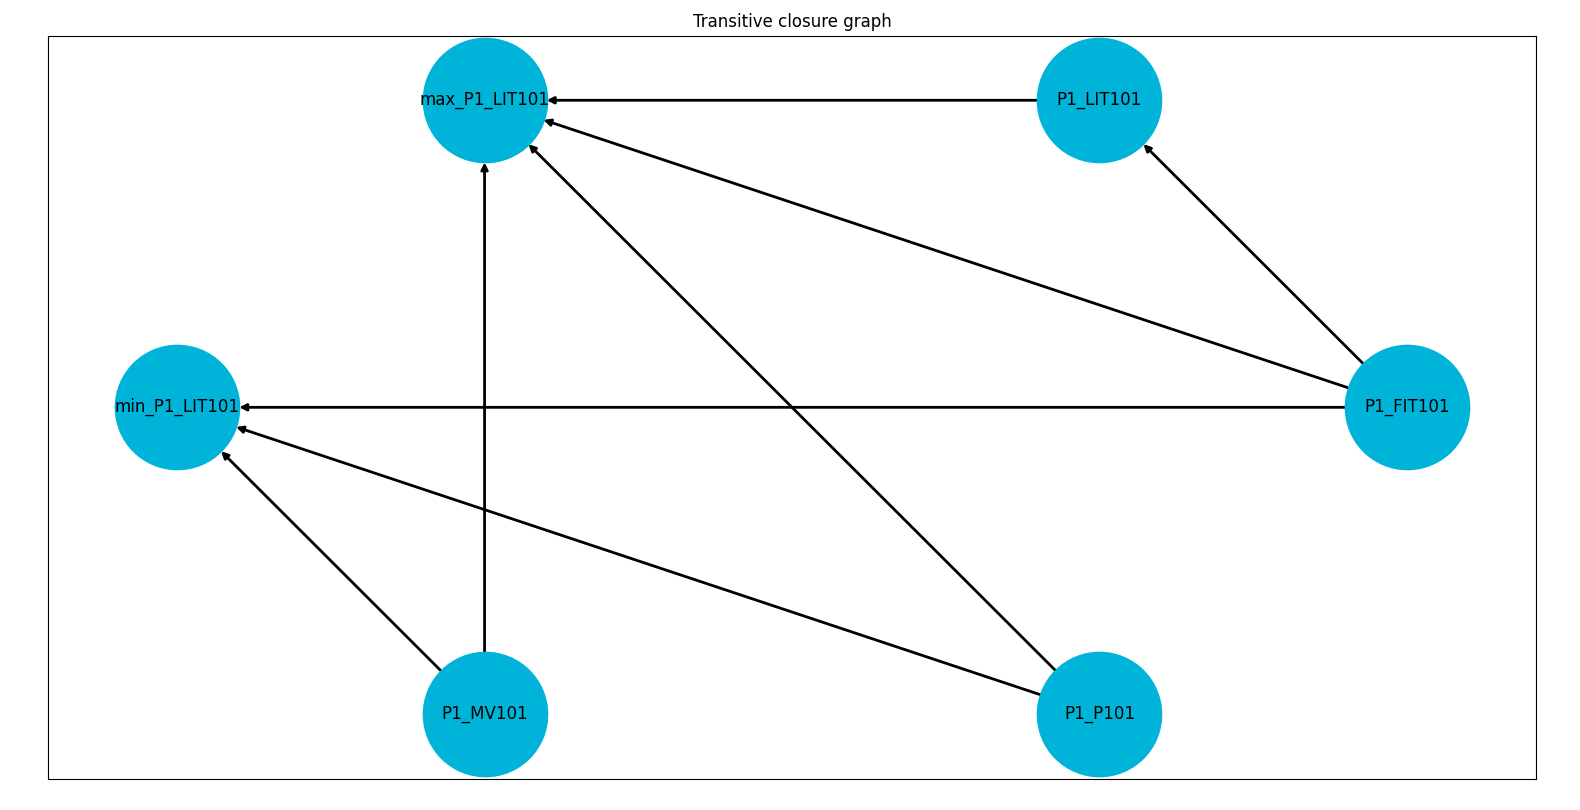
\includegraphics[width=\textwidth]{chap4/transitive_closure_lt.png}
		\caption{Transitive closure graph for "<"}
		\label{subfig:4_graph_lt}
	\end{subfigure}
	\hfill
	\begin{subfigure}{0.48\textwidth}
		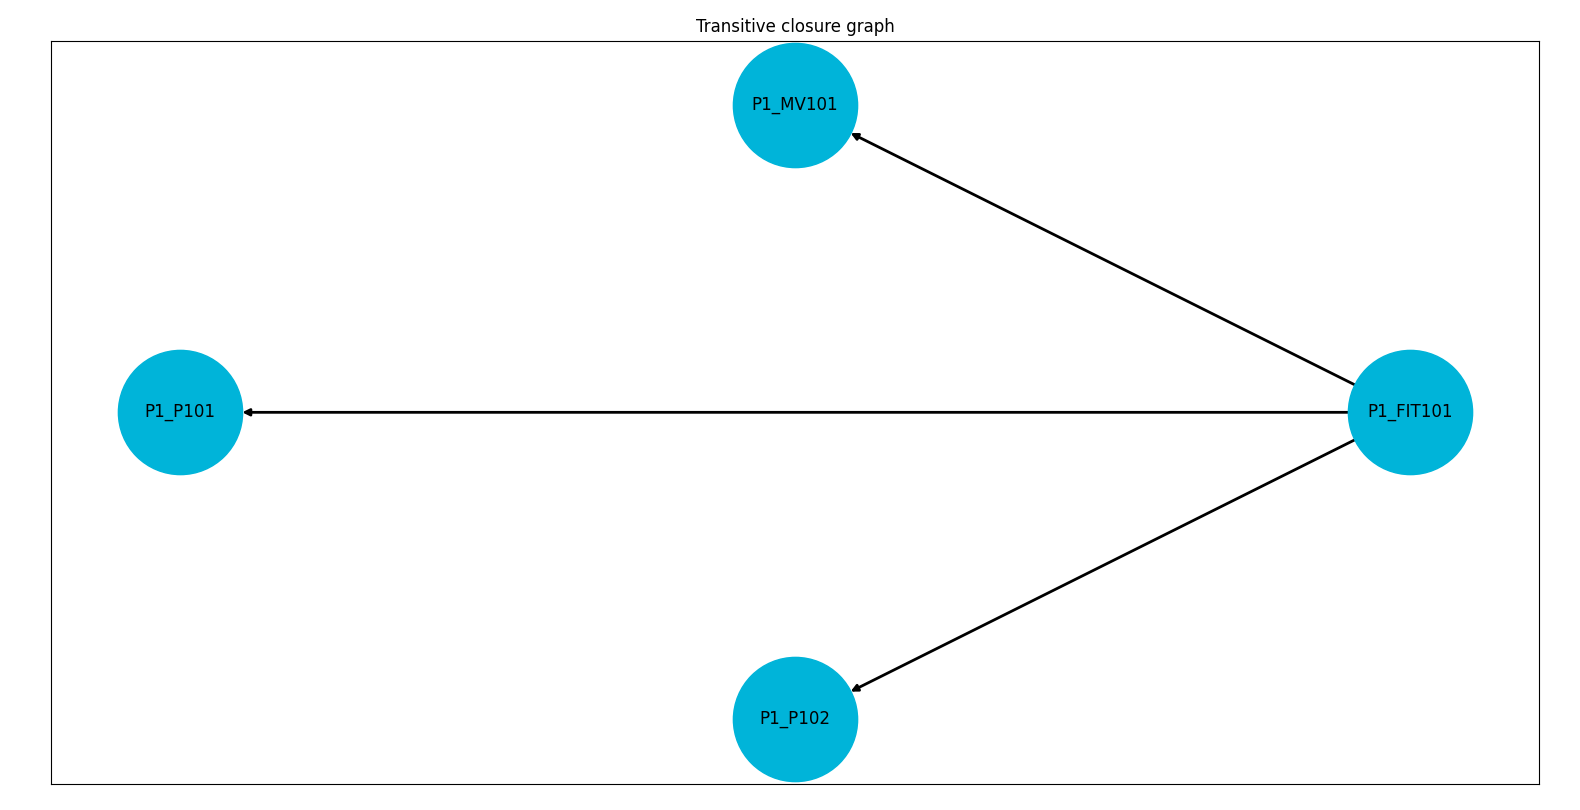
\includegraphics[width=\textwidth]{chap4/transitive_closure_gt_cond.png}
		\caption{Transitive closure graph for ">" cond.}
		\label{subfig:4_graph_gt_cond}
	\end{subfigure}
	\caption{Example of transitive closure graphs for invariants in PLC1 of iTrust SWaT system}
	\label{fig:4_transitive_closure_graphs}
\end{figure}
At the end of this process, still applied to \texttt{PLC1} of the iTrust SWaT system and with the same analysis condition, we get the following complete output:

\begin{lstlisting}[language=bash,numbers=left,caption={Revised Daikon output with transitive closures for \texttt{PLC1} of the iTrust SWaT system},label=lst:4_daikon_new_output_plc1]
	===========================
	Generic
	===========================
	P1_MV101 one of { 0.0, 1.0, 2.0 }
	P1_P101 one of { 1.0, 2.0 }
	slope_P1_LIT101 one of { -1.0, 0.0, 1.0 }
	P1_FIT101 != P1_P101, P1_P102
	P1_P102 == 1.0
	max_P1_LIT101 == 816.0
	min_P1_LIT101 == 489.0
	P1_LIT101 > P1_MV101
	P1_LIT101 > P1_P101
	P1_LIT101 > P1_P102
	P1_LIT101 > min_P1_LIT101 > slope_P1_LIT101
	P1_FIT101 >= 0.0
	P1_P101 >= P1_P102 >= slope_P1_LIT101
	
	===========================
	P1_MV101 == 2.0 && P1_LIT101 < max_P1_LIT101 - 16 && P1_LIT101 > min_P1_LIT101 + 15
	===========================
	slope_P1_LIT101 == P1_P102
	P1_MV101 == 2.0
	P1_FIT101 > P1_MV101
	P1_FIT101 > P1_P101
	P1_FIT101 > P1_P102
	P1_MV101 >= P1_P101
\end{lstlisting}
Transitive closures can be appreciated in lines 7, 14 and 16 of Listing \ref{lst:4_daikon_new_output_plc1}.\newline
In general, the output has been reduced in the number of effective rows (19 versus the 61 in the output of Listing \ref{lst:4_daikon_output_plc1}, making it certainly better to read and identify significant invariants) and the invariant chains make it more immediate to grasp the relationships between registers.
\vfill

\subsubsection{Types of Analysis}
\label{subsub:4_types_analysis}

Compared to Ceccato et al.'s solution, in which individual analyses are performed manually, my proposal is to implement two types of semi-automated analysis: the first performs an analysis of all states for each individual register, while the second performs the analysis on the current system configuration based on the actual states of the actuators.\newline
Both analyses refer to a specific measurement, selected by the user.

\bigskip
These two types of analysis will be handled by the Python script\\ \texttt{daikonAnalysis.py}, contained in the default directory \texttt{\$(project\_dir)/daikon}.\newline
The script accepts the following command-line arguments:

\begin{itemize}
	\item \textbf{-f} or \textbf{{-}{-}filename}: specifies the enriched dataset, in CSV format, from which to read the data. The dataset must be located within the directory containing the enriched datasets specified in the \textit{config.ini} file (by default \texttt{\$(project\_dir)/daikon/Daikon\_Invariants}).
	
	\item \textbf{-s} or \textbf{{-}{-}simpleanalysis}: performs the analysis on the states of individual actuators
	
	\item \textbf{-c} or \textbf{{-}{-}customanalysis}: performs the analysis on combinations of actual states of the actuators
	
	\item \textbf{-u} or \textbf{{-}{-}uppermargin}: defines a percentage margin on the maximum value of the measurement
	
	\item \textbf{-l} or \textbf{{-}{-}lowermargin}: defines a percentage margin on the minimum value of the measurement
\end{itemize}
One or both types of analysis can be selected. The last two parameters set a condition on the value of the measurement that is meant to bypass the transient periods between the actuator state change and the actual trend change at the maximum and minimum values: this expedient is especially useful for the first type of analysis, allowing for generally more accurate data on measurement trends.

\paragraph{Analysis on single actuator states}
Analysis on the states of individual actuators is the simplest: after the user is prompted to input the measurement, chosen from a list of likely available measurements, the script recognizes the likely actuators and the relative states of each, using the same mixed Daikon/Pandas technique adopted in the brief analysis during the pre-processing phase.\newline
For each actuator and each state it assumes, a single Daikon analysis is performed, eventually placing the condition on the maximum and minimum level of the measurement.\newline 
The result of these analyses are saved in the form of text files in a directory having the name corresponding to the analyzed actuator and contained in the default parent directory \texttt{\$(project\_dir)/daikon/Daikon\_Invariants/results}: each file generated by the analysis is identified by the name of the actuator, the state and the condition, if any, on the measurement (see Figure \ref{fig:4_daikon_simpleanalysis_dirfiles}).

\begin{figure}[H]
	\centering
	\begin{subfigure}{0.48\textwidth}
		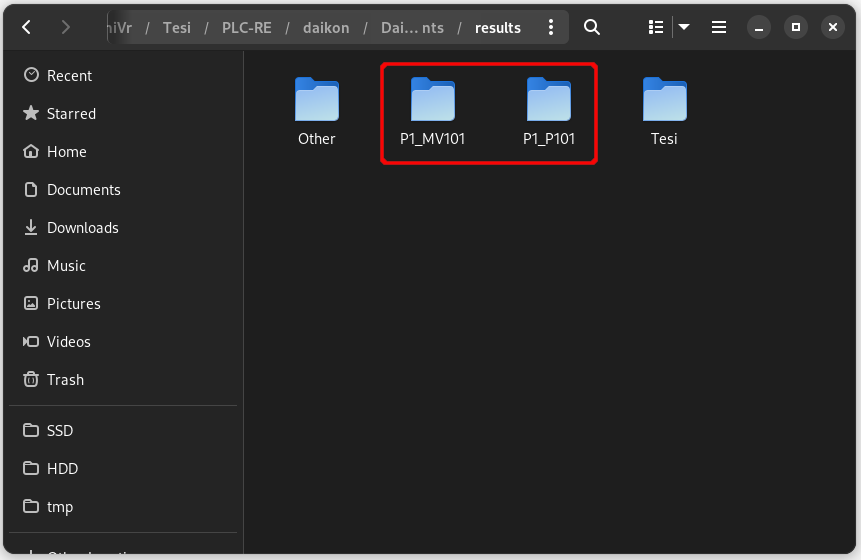
\includegraphics[width=\textwidth]{chap4/daikon_resultfiles_dirs.png}
		\caption{}
		\label{subfig:4_daikon_results_dir}
	\end{subfigure}
	\hfill
	\begin{subfigure}{0.48\textwidth}
		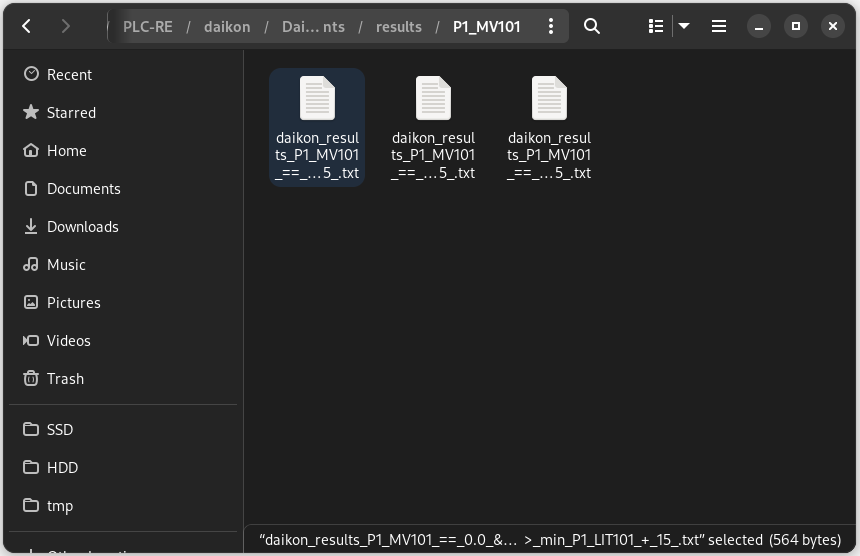
\includegraphics[width=\textwidth]{chap4/actuator_analysis_files.png}
		\caption{}
		\label{subfig:4_daikon_results_file}
	\end{subfigure}
	\caption{Directory (a) and outcome files (b) for the single actuator states analysis}
	\label{fig:4_daikon_simpleanalysis_dirfiles}
\end{figure}

An example of the outcome of this analysis is Listing \ref{lst:4_daikon_new_output_plc1}, where the actuator analyzed is \texttt{P1\_MV101} in state 2: from the generic invariants we can observe that \texttt{P1\_P101} is a likely actuator (line 5), assuming binary values; from line 8, however, we note that \texttt{P1\_P102} is permanently equal to 1, so it can be confirmed that it is a spare actuator rather than a setpoint; furthermore, lines 9 and 10 show the maximum and minimum values reached by \texttt{P1\_LIT101}, which we have assumed to be the register connected to the tank. The most interesting information, however, comes from the condition-generated invariants: at line 21 we notice that the slope of \texttt{P1\_LIT101} is 1 (thus increasing) when \texttt{P1\_MV101} is set to 2: this confirms what we assumed in the previous steps, namely, that \texttt{P1\_MV101} represents the ON state of the actuator and is responsible for filling the tank \texttt{P1\_LIT101}; moreover, at line 23 we see that \texttt{P1\_FIT101} is greater than \texttt{P1\_MV101}: this means that when the actuator assumes the value 2 the sensor \texttt{P1\_FIT101} detects data (in contrast, if \texttt{P1\_MV101} is 1 \texttt{P1\_FIT101} is 0, detecting nothing), confirming the original hypothesis made that this may be a pressure or flow sensor.

\paragraph{Analysis of the Current System Configuration}
The analysis of the current system configuration based on the actual states of the actuators is more complex, but at the same time offers more interesting outcomes as it provides better evidence of actuator behavior in relation to the selected measurement.

\begin{figure}[H]
	\centering
	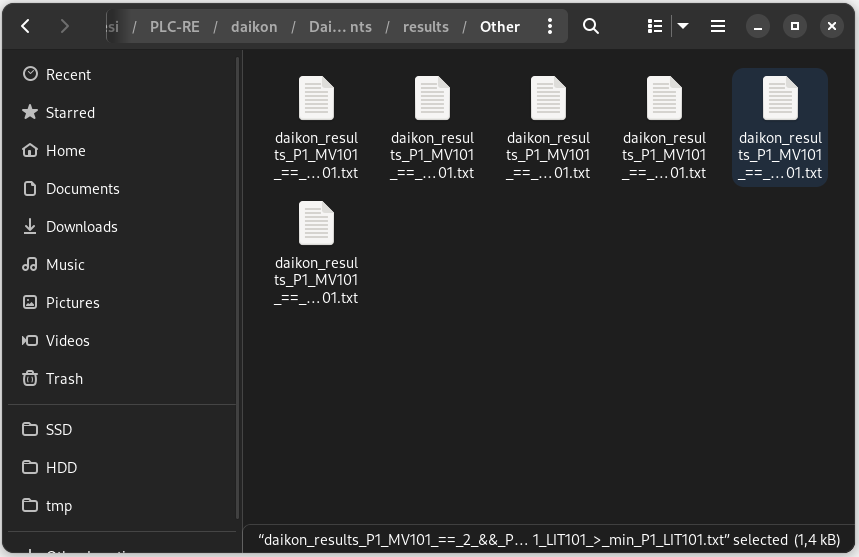
\includegraphics[scale=0.35]{chap4/daikon_systemstate_results.png}
	\caption{Daikon outcome files for system configuration analysis. Each file represents a single system state}
	\label{fig:4_daikon_systemstates_files}
\end{figure}

For this analysis, the script automatically recognizes the actual configurations of the actuators (e.g., \texttt{P1\_MV101 == 2, P1\_P101 == 1}) that represent a system state, and for each of these configurations  Daikon analysis is automatically run, after prompting the user for the measurement and eventually the actuators whose configurations are to be studied (If the user does not select any actuators, all those previously detected by the Python script will be considered): the analysis outcomes are saved, still in the text format, within a specific directory under the same parent directory of the previous type of analysis and, as before, their name is characterized by the rule used for the analysis (see Figure \ref{fig:4_daikon_systemstates_files}).\newline \newline
An example of the obtained outcomes can be seen in Listing \ref{lst:4_current_system_config_analysis}:

\begin{lstlisting}[language=bash,numbers=left,caption={Daikon outcomes for the system configuration \texttt{P1\_MV101 == 2, P1\_P101 == 1} on \texttt{P1\_LIT101}},label=lst:4_current_system_config_analysis]
	===========================
	Generic
	===========================
	P1_MV101 <= P1_P101  ==>  P1_FIT101 >= 0.0
	P1_MV101 <= P1_P101  ==>  P1_MV101 one of { 0.0, 1.0, 2.0 }
	P1_MV101 <= P1_P101  ==>  P1_P101 one of { 1.0, 2.0 }
	P1_MV101 <= P1_P101  ==>  slope_P1_LIT101 one of { -1.0, 0.0, 1.0 }
	P1_MV101 > P1_P101  ==>  P1_FIT101 > P1_MV101
	P1_MV101 > P1_P101  ==>  P1_FIT101 > P1_P101
	P1_MV101 > P1_P101  ==>  P1_FIT101 > P1_P102
	P1_MV101 > P1_P101  ==>  P1_FIT101 > slope_P1_LIT101
	P1_MV101 > P1_P101  ==>  P1_MV101 == 2.0
	P1_MV101 > P1_P101  ==>  P1_MV101 > P1_P102
	P1_MV101 > P1_P101  ==>  P1_MV101 > slope_P1_LIT101
	P1_MV101 > P1_P101  ==>  P1_P101 == 1.0
	P1_MV101 > P1_P101  ==>  P1_P101 == P1_P102
	P1_MV101 > P1_P101  ==>  P1_P101 == slope_P1_LIT101
	P1_MV101 > P1_P101  ==>  slope_P1_LIT101 == 1.0
	[...]
	
	===========================
	P1_MV101 == 2 && P1_P101 == 1 && P1_LIT101 < max_P1_LIT101 && P1_LIT101 > min_P1_LIT101
	===========================
	slope_P1_LIT101 == P1_P102 == P1_P101 == 1.0
	P1_MV101 == 2.0
	P1_FIT101 > P1_MV101
	P1_FIT101 > P1_P101
\end{lstlisting}
Compared to Listing \ref{lst:4_daikon_new_output_plc1}, this time we can observe in the general invariants section the presence of implications, which were previously absent (the remaining generic invariants have been omitted for reasons of space). Such implications can provide very useful information, as in this case: for example, the invariant on line 18 tells us that if the value of \texttt{P1\_MV101} is greater than that of \texttt{P1\_P101} then the value of the slope is 1, that is, the tank level is increasing. Consequently, we have further confirmation that the state \texttt{P1\_MV101 == 2} is the ON state for that actuator and that it is the actuator responsible for filling the tank \texttt{P1\_LIT101}. Comparing the other analysis outcomes, we will discover that \texttt{P1\_P101} is instead responsible for emptying the tank and that its ON and OFF states are 2 and 1, respectively.\newline
In addition, the invariant at line 8 also indicates that when the actuator \texttt{P1\_MV101} is in state 2 and \texttt{P1\_P101} is in state 1 then the value of \texttt{P1\_FIT101} is greater than 2: consequently, it follows that the corresponding sensor is measuring something relative to the tank \texttt{P1\_LIT101}.\newline
The above is confirmed by the invariants related to the analysis condition: at line 24 we have that the slope is indeed equal to 1 (thus increasing) and that \texttt{P1\_FIT101}, at line 26, takes values greater than 2 when \texttt{P1\_MV101} is equal to 2.

\paragraph{Refining the Analysis}
In some cases, it may happen that the outcomes provided by the semi-automated analyses are not satisfactory to the user (e.g., the value of the slope may not emerge clearly) or simply the user wants to investigate a particular aspect of the system in more detail by trying to discover additional invariants that did not emerge previously: in this case, it is possible to run a new and more specific invariant analysis using the Python script \texttt{runDaikon.py}, which allows for more punctual analyses of the system.\newline
The script, also contained in the default directory \texttt{\$(project\_dir)/daikon}, accepts three command-line parameters:

\begin{itemize}
	\item \textbf{-f} or \textbf{{-}{-}filename}: specifies the enriched dataset, in CSV format, from which to read the data. Even in this case, the dataset must be located within the directory containing the enriched datasets
	\item \textbf{-c} or \textbf{{-}{-}condition}: specifies the condition for the analysis, which will be automatically overwritten in the \textit{.spinfo} file. It is possible to specify more than one condition, but it is recommended to use the logical operator \texttt{\&\&}
	\item \textbf{-r} or \textbf{{-}{-}register}: specifies the directory where to save the text file with the outcomes
\end{itemize}
Performing this single analysis will produce a single output file containing the invariants discovered, file that will be saved in the directory specified by the user via the \texttt{-r} command-line option (by default the file will be saved in the directory \texttt{\$(project\_dir)/daikon/Daikon\_Invariants/results}) to be examined later by the user.

\bigskip
In conclusion, the two types of analysis presented, along with the possibility of allowing for more refined analysis at a later date and Daikon's redefined output, make this stage much more complete, clear, and powerful than before

\subsection{Phase 4: Businness Process Analysis}
\label{subsec:4_improve_bpa}

\vfill
\nolinenumbers